% !TeX root = ../../Book1.tex
% 纲要标题：## 第10章　非 Euclid 模型、离散作用与几何结构
% 纲要位置：几何学计划纲要.md，第 501 行。
% 正文状态：初稿；尚未正式审核。

% 纲要内容开始
% 
% > 本章目标与证明范围：保留球面与双曲几何的独立深入模块。先计算模型，再研究离散群商与局部齐性结构；一般统一化是第四卷的后续任务，不从模型存在直接推出。
% 
% 纲要内容结束

\chapter{非 Euclid 模型、离散作用与几何结构}
\label{g1:ch:10}
\BookChapterNumber{g1:ch:10}

\begin{chapterabstract}
	常曲率曲面既可以用具体公式计算，也可以作为局部几何的标准模型。本章构造双曲面、圆盘和上半平面之间的等距映射，求距离、测地线、等距群及球面与双曲三角恒等式，并把角和与面积相联系。随后从等距变换的分类研究离散作用，证明自由固有作用的商结构，按边和顶点的实际条件粘合基本多边形，构造闭双曲曲面、尖点与漏斗。最后沿道路延续几何坐标，建立展开映射与单值表示，并证明完备模型结构与模型商之间的关系。
\end{chapterabstract}

\begin{learninggoals}
	\begin{itemize}
		\item 在三种双曲模型之间明确转换点、切向量、度量和测地线，区分 Euclid 图形与模型中的长度、角度。
		\item 推导球面和双曲三角公式，利用曲率归一化计算面积，判定正则测地多边形的角条件。
		\item 用固定点、矩阵迹和标准型区分椭圆、抛物与双曲变换，判断离散性、自由性和固有性的作用。
		\item 检查边配对的长度匹配、顶点链接和总角，构造具有光滑双曲度量的闭曲面及其典型非紧端。
		\item 从几何图册构造展开映射，核对单值表示的乘法顺序与等变性，说明完备性如何保证整体商的实现。
	\end{itemize}
\end{learninggoals}

在 Euclid 平面里，三角形的三个角之和总是 \(\pi\)。球面上的短大圆三角形却有更大的角和；第九章说明，多出来的角恰好记录它围住的曲率积分。那么，角和小于 \(\pi\) 的几何能否同样明确地计算？如果把许多这样的图形按边粘合，怎样保证接缝和顶点附近仍是同一种光滑几何？这些问题把局部的测量公式与整张曲面的构造联系起来。

\ProseParagraphBreak

双曲几何有几种外观差别很大的模型。上半平面中，靠近实轴的一小段 Euclid 距离可能对应很长的双曲距离；圆盘中的测地线通常画成圆弧；双曲面则把距离计算转为一个带负号的双线性型。证明模型间的等距，才能在最便于眼前计算的模型中工作。它们的理想边界也需要与通常的度量边界分清：图中看得见的边缘，并不是走有限长度便能抵达的缺口。

\ProseParagraphBreak

研究商空间时，局部模型仍不够。一个群可以离散却有固定点，配对的边也可以等长却在顶点留下锥形奇点。我们逐项核对这些条件，再将问题反过来：如果只知道每一小块都具有同样的几何，能否把整张曲面放回一个标准模型中？展开映射先回答万有覆盖上的延续问题；单值表示记录绕路后的坐标变化；完备性则负责排除有限长度处中断的情形。这里的结构单值与第九章切向量的环路平行移动变换有不同的对象和作用，使用时会加以区分。

\ProseParagraphBreak

本章使用有限维线性代数、多元微积分与复数运算，复数只作为平面坐标及分式变换的记法。第五章的覆盖与道路拼接、第六章的曲面边配对、第九章的测地邻域与 Gauss--Bonnet 公式在调用处恢复所需条件。进一步阅读可查 Ratcliffe 第三版：球面、双曲模型及三角计算见\cite[\S\S~2.3--2.5, 3.1--3.5, 4.3--4.6]{Ratcliffe2019}；离散作用、基本区域和曲面粘合见\cite[\S\S~4.7, 5.2--5.3, 6.6, 9.2, 9.7--9.8]{Ratcliffe2019}；展开与完备性见\cite[\S\S~8.3--8.5]{Ratcliffe2019}。本章构造具体的常曲率结构，并证明给定完备结构的商描述；一般统一化仍属于第四卷的后续内容。

% !TeX root = ../../Book1.tex
% 纲要标题：### 10.1 常曲率模型的度量几何
% 纲要位置：几何学计划纲要.md，第 505 行。
% 正文状态：初稿；尚未正式审核。

% 纲要内容开始
% 
% * 双曲面、圆盘和上半平面
% * 模型间等距映射的构造
% * 距离、测地线及理想边界
% * Möbius 变换与等距群
% * 球面与双曲三角恒等式
% * 角和、面积及曲率归一化
% * 测地多边形和角条件
% 
% 纲要内容结束

\section{常曲率模型的度量几何}
\label{g1:sec:1001}

同样是圆盘，在通常的欧氏度量下，走到边缘只需有限长度；若越靠近边缘，度量把长度放大得越快，边缘就可能变得无限遥远。双曲平面的圆盘模型正是这样的例子。为了看清距离、测地线和对称变换，我们还会把同一几何放在双曲面与上半平面中表达。三个模型各有便于计算的地方，彼此间的显式等距映射使这些计算能够相互转用。

\subsection{双曲面、圆盘和上半平面}
\label{g1:subsec:1001:01}

先取单位球面 \(S^2\subset\mathbb R^3\) 及其诱导度量，它的曲率为 \(1\)。我们寻找一个负曲率的对应模型。把通常内积中的一项改成负号，定义 \(\mathbb R^3\) 上的双线性型
\[
	\langle x,y\rangle_L\coloneqq-x_0y_0+x_1y_1+x_2y_2.
\]
这是\term[lorentzxing]{Lorentz 型}[Lorentzian form]，不是正定内积；例如 \(\langle(1,0,0),(1,0,0)\rangle_L=-1\)。我们并不把它在整个 \(\mathbb R^3\) 上当作长度，而只将它限制到下面曲面的切平面。\footnote{Lorentz，中文常译洛伦兹；Hendrik Antoon Lorentz（1853--1928），荷兰理论物理学家，研究电磁理论、电子理论与运动物体的变换。}

\begin{definition}
	\label{g1:def:hyperbolic-models}
	\term[shuangqumianmoxing]{双曲面模型}[hyperboloid model]是
	\[
		\mathbb H_L^2\coloneqq\{x:\langle x,x\rangle_L=-1,\ x_0>0\},
		\qquad g_L(v,w)=\langle v,w\rangle_L.
	\]
	另外定义\term[yuanpanmoxing]{圆盘模型}[disc model]与\term[shangbanpingmianmoxing]{上半平面模型}[upper half-plane model]：
	\begin{align*}
		\mathbb D&=\{w=u+iv:|w|<1\},&
		g_{\mathbb D}&=\frac{4(\mathrm{d}u^2+\mathrm{d}v^2)}{(1-|w|^2)^2},\\
		\mathbb H&=\{z=x+iy:y>0\},&
		g_{\mathbb H}&=\frac{\mathrm{d}x^2+\mathrm{d}y^2}{y^2}.
	\end{align*}
	复数记号 \(|\mathrm{d}z|^2\) 只简写实二次型 \(\mathrm{d}x^2+\mathrm{d}y^2\)。后两个模型采用平面的标准定向。
\end{definition}

双曲面上的度量确实正定。写 \(x=(x_0,x')\)，则 \(x_0=\sqrt{1+|x'|^2}\)，所以它首先是一个光滑图像。切向量 \(v=(v_0,v')\) 满足 \(x_0v_0=x'\cdot v'\)，从而
\[
	\langle v,v\rangle_L=|v'|^2-\frac{(x'\cdot v')^2}{x_0^2}
	\geq\frac{|v'|^2}{x_0^2}>0\qquad(v\ne0).
\]
这里最后一个严格不等式来自：若 \(v'=0\)，切向条件也使 \(v_0=0\)。因此这个不定型在每个切平面上都给出通常意义的正定长度与角度。它与双曲面作为欧氏空间曲面时的诱导度量不同，不能用欧氏空间中该图像的主曲率代替它的内在曲率。

\ProseParagraphBreak

在上半平面上，\(g_{\mathbb H}=e^{2\phi}(\mathrm{d}x^2+\mathrm{d}y^2)\)，其中 \(\phi=-\log y\)。回忆\eqref{g1:eq:conformal-gauss-curvature}，共形度量的曲率为 \(-e^{-2\phi}(\phi_{xx}+\phi_{yy})\)。这里 \(\phi_{xx}=0\)、\(\phi_{yy}=1/y^2\)，故 \(K=-1\)。圆盘与双曲面是否也给出相同几何，需要下一小节的等距计算，而不能只凭外形或名称判断。

\subsection{模型间等距映射的构造}
\label{g1:subsec:1001:02}

从点 \((-1,0,0)\) 向平面 \(x_0=0\) 投影，会把双曲面上半支送到单位圆盘。这一选择中的 \(-1\) 使投影分母始终为正，也让无穷远处趋向圆周。上半平面到圆盘则用一个把实轴变成圆周的分式映射。

\begin{proposition}[三个模型的等距]
	\label{g1:prop:hyperbolic-model-isometries}
	以下映射均为光滑等距微分同胚：
	\begin{align*}
		P:\mathbb H_L^2&\longrightarrow\mathbb D,&
		P(x)&=\frac{x_1+ix_2}{x_0+1},\\
		C:\mathbb H&\longrightarrow\mathbb D,&
		C(z)&=\frac{z-i}{z+i}.
	\end{align*}
	双曲面的定向取为使 \(P\) 保向的定向；\(C\) 也保持定向。因此三个模型都具有常曲率 \(-1\)，统称为\term[shuangqupingmian]{双曲平面}[hyperbolic plane]。
\end{proposition}
\begin{proof}
	先由 \(x_1^2+x_2^2=x_0^2-1\)，得到 \(|P(x)|^2=(x_0-1)/(x_0+1)<1\)。反解为
	\[
		P^{-1}(u+iv)=\frac{(1+u^2+v^2,\,2u,\,2v)}{1-u^2-v^2}.
	\]
	这给出了互逆的光滑映射。记 \(q=1-u^2-v^2\)、\(a=u\,\mathrm{d}u+v\,\mathrm{d}v\)。对逆映射求导，有
	\[
		\mathrm{d}x_0=\frac{4a}{q^2},\qquad
		\mathrm{d}(x_1,x_2)=\frac{2(\mathrm{d}u,\mathrm{d}v)}q+\frac{4(u,v)a}{q^2}.
	\]
	代入 Lorentz 型，含 \(a^2\) 的系数为 \(16/q^3+16(u^2+v^2-1)/q^4=0\)，剩下 \(4(\mathrm{d}u^2+\mathrm{d}v^2)/q^2\)，正是圆盘度量。

	对 \(C\)，直接算得
	\[
		1-|C(z)|^2=\frac{4y}{|z+i|^2},\qquad
		C'(z)=\frac{2i}{(z+i)^2},\qquad C^{-1}(w)=i\frac{1+w}{1-w}.
	\]
	这些式子证明 \(C\) 恰把上半平面双射到圆盘，且正反映射光滑。复导数乘法把实长度放大 \(|C'(z)|\) 倍，故
	\[
		C^*g_{\mathbb D}
		=\frac{4|C'(z)|^2|\mathrm{d}z|^2}{(1-|C(z)|^2)^2}
		=\frac{|\mathrm{d}z|^2}{y^2}.
	\]
	非零复数乘法的实行列式为其模平方，所以 \(C\) 保向。最后，等距保持内在曲率，这是\cref{g1:thm:theorema-egregium}及其度量表达\eqref{g1:eq:intrinsic-gauss-curvature}的结论，故三个模型的曲率都是 \(-1\)。
\end{proof}

这些坐标图的用途不同：双曲面的线性代数适合距离与三角公式，圆盘适合展示对称性，上半平面的分式变换适合研究群作用。圆盘和上半平面的度量都是欧氏度量乘以一个正函数，因而保留欧氏角度；它们并不保留欧氏长度。

\subsection{距离、测地线及理想边界}
\label{g1:subsec:1001:03}

在连通度量曲面上，用全部连接 \(p,q\) 的分片 \(C^1\) 曲线定义长度距离
\[
	d(p,q)\coloneqq\inf_{\gamma:p\to q}L(\gamma).
\]
三角不等式来自道路拼接，反向参数给出对称性。局部坐标中的正定度量在小闭坐标球上有正的下界，故走出这个球需要正长度，这也保证不同点的距离不为零。前章的径向极小定理只在正常邻域内比较短曲线；对双曲平面，可以利用模型把比较推广到任意两点。

\begin{theorem}[双曲距离与测地线]
	\label{g1:thm:hyperbolic-distance-geodesics}
	双曲面模型中，若 \(p\in\mathbb H_L^2\)、\(v\in \mathrm{T}_p\mathbb H_L^2\) 且 \(\langle v,v\rangle_L=1\)，则所有单位速测地线由
	\begin{equation}
		\label{g1:eq:hyperboloid-geodesic}
		\gamma(t)=p\cosh t+v\sinh t,\qquad t\in\mathbb R
	\end{equation}
	给出。任意两个不同点之间有唯一测地线段，并且它在全部分片 \(C^1\) 连接曲线中最短。三个模型中的距离分别满足
	\begin{align}
		\cosh d(p,q)&=-\langle p,q\rangle_L,
		\label{g1:eq:hyperboloid-distance}\\
		\cosh d(w_1,w_2)&=1+\frac{2|w_1-w_2|^2}{(1-|w_1|^2)(1-|w_2|^2)},
		\label{g1:eq:disc-distance}\\
		\cosh d(z_1,z_2)&=1+\frac{|z_1-z_2|^2}{2\operatorname{Im}z_1\operatorname{Im}z_2}.
		\label{g1:eq:half-plane-distance}
	\end{align}
	双曲平面单连通，其长度距离完备，每个闭有界球紧；每条测地线也都能在整个实数轴上延拓。
\end{theorem}
\begin{proof}
	先说明如何把任意点移到 \(o=(1,0,0)\)。空间坐标 \((x_1,x_2)\) 的旋转保持 Lorentz 型，而矩阵
	\[
		B_r=\begin{pmatrix}\cosh r&\sinh r&0\\\sinh r&\cosh r&0\\0&0&1\end{pmatrix}
	\]
	也保持该型，并把 \(o\) 送到 \((\cosh r,\sinh r,0)\)。任意点都能写成
	\[
		x=(\cosh r,\sinh r\cos\theta,\sinh r\sin\theta),
	\]
	所以这些变换在双曲面上传递；它们保持上半支，因为变换后的第零坐标不可能为零，且上半支连通。其微分保持切平面上的度量，故都是等距。

	双曲面的协变导数可以由 Lorentz 正交投影计算：沿 \(\gamma\) 的切向量场 \(W\) 满足
	\[
		\mathrm{D}_tW=\dot W+\langle\dot W,\gamma\rangle_L\gamma.
	\]
	右边确与 \(\gamma\) 正交；逐项求导内积给出度量相容，交换坐标导数给出无挠性，因此\cref{g1:prop:surface-connection-properties}的唯一性说明它就是度量联络。对单位速曲线，\(\langle\ddot\gamma,\gamma\rangle_L=-1\)，故测地线方程等价于 \(\ddot\gamma=\gamma\)。解这个线性方程即得\eqref{g1:eq:hyperboloid-geodesic}；代入可核验它始终位于上半支且速度为 \(1\)。前章\cref{g1:prop:geodesic-initial-values}的唯一性说明没有遗漏同初值的其他测地线。

	以 \(o\) 为中心，上面的径向参数给出
	\begin{equation}
		\label{g1:eq:hyperbolic-polar-metric}
		g_L=\mathrm{d}r^2+\sinh^2r\,\mathrm{d}\theta^2,\qquad r>0.
	\end{equation}
	这是直接微分 \((\cosh r,\sinh r\cos\theta,\sinh r\sin\theta)\) 所得。任何从 \(o\) 到径向坐标 \(r_0\) 的曲线，其速度不小于径向速度的绝对值。为避开 \(r=0\) 的极坐标奇点，取 \(0<\varepsilon<r_0\)，只比较曲线最后一次离开 \(r=\varepsilon\) 后的一段，得到长度至少为 \(r_0-\varepsilon\)；让 \(\varepsilon\) 趋零，便得下界 \(r_0\)。固定 \(\theta\) 的径向测地段达到该下界。

	将任意起点 \(p\) 等距移到 \(o\)，可知两点间距离是 \(\operatorname{arcosh}(-\langle p,q\rangle_L)\)。当 \(p\ne q\) 时记它为 \(a>0\)，则到达 \(q\) 的单位初速度必须是
	\[
		v=\frac{q-p\cosh a}{\sinh a}.
	\]
	该向量与 \(p\) 正交且 Lorentz 长度为 \(1\)，于是相应测地段存在且唯一。双曲面测地线的轨迹是过原点的二维平面与上半支之交，且每条单位速参数线都不重复。将 \(P^{-1}\) 代入 Lorentz 内积，整理即得\eqref{g1:eq:disc-distance}；再用
	\[
		|C(z_1)-C(z_2)|^2=\frac{4|z_1-z_2|^2}{|z_1+i|^2|z_2+i|^2}
	\]
	及上一小节的 \(1-|C(z)|^2\) 公式，得到\eqref{g1:eq:half-plane-distance}。

	由距离公式，\(o\) 的半径 \(R\) 闭球恰是双曲面上 \(x_0\leq\cosh R\) 的部分，它在 \(\mathbb R^3\) 中闭且有界，故紧。距离公式又说明坐标收敛蕴含距离收敛；反过来，将极限点移到 \(o\)，由 \(x_0=\cosh r\)、\(|x'|=\sinh r\) 可知距离收敛蕴含坐标收敛。因此上述紧性也是长度距离的紧性。任意 Cauchy 序列有界，落在某个这样的紧球内，有收敛子列，再由 Cauchy 条件整个序列收敛，故度量完备。公式\eqref{g1:eq:hyperboloid-geodesic}另已直接给出测地线的全时延拓；这里没有把两种完备性未经证明地互换。最后，圆盘凸且可沿直线缩到原点，故单连通，模型间的微分同胚将这一性质传给双曲面和上半平面。
\end{proof}

圆盘中的测地线是直径或与单位圆周正交的圆弧。具体地，双曲面测地线所在平面可写为 \(a_0x_0+a_1x_1+a_2x_2=0\)，投影后成为
\[
	a_0(1+u^2+v^2)+2a_1u+2a_2v=0.
\]
当 \(a_0=0\) 时是过原点的直线；否则圆心为 \((-a_1/a_0,-a_2/a_0)\)，半径平方等于圆心到原点距离平方减去 \(1\)，这正是与单位圆正交的条件。每条相交圆弧都对应一个这样的测地平面。把 \(w=C(z)\) 代入，方程化成 \(A(x^2+y^2)+Bx+C_0=0\)，所以在上半平面中，它们是以实轴上点为圆心的半圆，或垂直实轴的直线。通过两个不同内点的这类弧唯一，正与定理的唯一性一致。

\begin{figure}[htbp]
	\centering
	% !TeX root = ../Book1.tex
\begin{tikzpicture}[>=stealth,font=\small]
	\begin{scope}[yshift=1.5cm]
		\draw[dashed,gray] (0,0) circle (1.5);
		\draw[blue!70!black,thick] (-1.5,0)--(1.5,0);
		\draw[blue!70!black,thick] ({1.5*cos(55)},{1.5*sin(55)}) arc[start angle=145,end angle=215,radius={1.5*tan(55)}];
		\fill[gray] ({1.5*cos(55)},{1.5*sin(55)}) circle (1.3pt);
		\fill[gray] ({1.5*cos(55)},{-1.5*sin(55)}) circle (1.3pt);
		\node[above left] at (-.9,1.25) {\(\partial_\infty\mathbb H^2\)};
		\node at (0,-1.95) {圆盘模型};
	\end{scope}
	\draw[->] (3.05,1.55)--(2.05,1.55) node[midway,above] {\(C\)};
	\begin{scope}[xshift=5cm]
		\draw[dashed,gray,->] (-1.65,0)--(1.7,0) node[right] {\(\mathbb R\)};
		\draw[blue!70!black,thick] (-1.35,0) arc[start angle=180,end angle=0,radius=1.05];
		\draw[blue!70!black,thick,->] (1.05,0)--(1.05,2.75) node[above] {\(\infty\)};
		\fill[gray] (-1.35,0) circle (1.3pt);
		\fill[gray] (.75,0) circle (1.3pt);
		\fill[gray] (1.05,0) circle (1.3pt);
		\node at (0,-.45) {上半平面模型};
	\end{scope}
\end{tikzpicture}

	\caption[双曲平面的测地线与理想边界]{圆盘中的测地线为直径及正交于圆周的圆弧；上半平面中则为垂直实轴的直线及圆心在实轴上的半圆。灰色边界用于表示理想端点，不属于模型本身。图中的两组曲线分别示意各模型中的形状，不标示逐条对应。}
	\label{g1:fig:hyperbolic-model-geodesics}
\end{figure}

圆盘的圆周称为其\term[lixiangbianjie]{理想边界}[ideal boundary]，记为 \(\partial_\infty\mathbb H^2\)。上半平面的相应边界是 \(\mathbb R\cup\{\infty\}\)，其中一点 \(\infty\) 由 \(C\) 送到圆周上的 \(1\)。理想端点只描述测地线向哪个方向无限延伸，不是度量完备化中缺少的点。事实上
\[
	d_{\mathbb D}(0,w)=2\operatorname{artanh}|w|
	=\log\frac{1+|w|}{1-|w|}\longrightarrow\infty\qquad(|w|\to1).
\]
双曲面上，同一个端点由向量 \(p+v\) 的正比例类表示，因为\eqref{g1:eq:hyperboloid-geodesic}在 \(t\to+\infty\) 时沿 \(e^t(p+v)/2\) 增长，而 \(\langle p+v,p+v\rangle_L=0\)。不同理想端点恰好确定一条完整测地线；在上半平面中，两有限端点决定一个半圆，有一个端点为 \(\infty\) 时则决定一条竖线。

\ProseParagraphBreak

球面的距离提供了重要对照。\cref{g1:exm:sphere-geodesics}已证明单位球面的测地线是大圆，而且可全时延拓。固定 \(p\in S^2\)，写 \(q=p\cos r+u\sin r\)，其中 \(u\perp p\)、\(|u|=1\)、\(0<r<\pi\)。直接微分给出 \(\mathrm{d}r^2+\sin^2r\,\mathrm{d}\theta^2\)，同样的径向长度比较得到
\begin{equation}
	\label{g1:eq:spherical-distance}
	d_{S^2}(p,q)=\arccos(p\cdot q)\in[0,\pi].
\end{equation}
到对径点时可先截到 \(r=\pi-\varepsilon\) 再取极限，故同一公式仍成立。非对径的不同点之间，较短大圆弧是唯一最短测地段；对径点之间所有半大圆都最短。距离公式还说明它与球面原有拓扑相同，因此球面的紧性保证度量完备以及闭球紧。球面单连通已由\cref{g1:prop:sphere-simply-connected}证明；欧氏平面的相应三种性质则分别来自凸性、欧氏 Cauchy 序列收敛和闭有界集紧性。

\subsection{Möbius 变换与等距群}
\label{g1:subsec:1001:04}

已经知道模型之间怎样等距，现在要找同一模型的全部等距。仅写出一族保持度量的公式还不够，还须证明没有遗漏。一个实用的办法是先证明：等距只要在一点具有相同的位置和微分，便处处相同；随后用显式变换实现所有可能的初始数据。

\begin{proposition}[等距的初始数据]
	\label{g1:prop:isometry-initial-data}
	设 \(M,N\) 是光滑度量曲面，\(M\) 连通，\(F_1,F_2:M\to N\) 为局部等距。若在某一点 \(p\) 有 \(F_1(p)=F_2(p)\) 且 \(\mathrm{d}(F_1)_p=\mathrm{d}(F_2)_p\)，则 \(F_1=F_2\)。特别地，两个局部等距若在非空开集上相同，就在其连通公共定义域上相同。
\end{proposition}
\begin{proof}
	局部等距保持联络：在可逆邻域上，把目标联络拉回源曲面，所得运算满足度量相容、无挠性及求导法则，故由\cref{g1:prop:surface-connection-properties}的唯一性，等于源联络。因此它把带原仿射参数的测地线映为测地线。\cref{g1:prop:geodesic-initial-values}的初值唯一性给出
	\[
		F_i(\exp_qv)=\exp_{F_i(q)}\bigl(\mathrm{d}(F_i)_qv\bigr)
	\]
	对充分小的 \(v\) 成立。

	令 \(S\) 为两映射的位置与微分都相同的点集。假设使它非空。若 \(q\in S\)，由\cref{g1:prop:normal-neighborhood}，\(\exp_q\) 在零附近给出一个开邻域坐标，上式使两映射在整个邻域相同，其微分自然也相同，故 \(S\) 开。若 \(q_j\in S\) 且 \(q_j\to q\)，连续性先给出 \(F_1(q)=F_2(q)\)；在该公共像点附近选一张坐标图，再用两映射的一阶导数连续性，得到 \(\mathrm{d}(F_1)_q=\mathrm{d}(F_2)_q\)，故 \(S\) 闭。连通性迫使 \(S=M\)。
\end{proof}

以下的等距指保持度量的光滑微分同胚，组成等距群 \(\operatorname{Isom}\)。取实矩阵 \(A=\begin{psmallmatrix}a&b\\c&d\end{psmallmatrix}\) 且 \(ad-bc=1\)，定义\term[mobiusbianhuan]{Möbius 变换}[Möbius transformation]
\[
	f_A(z)=\frac{az+b}{cz+d}.
\]
分母在上半平面不为零。其在实轴及 \(\infty\) 上的取值按分式极限解释，例如 \(c\ne0\) 时 \(f_A(\infty)=a/c\)。

\begin{theorem}[双曲平面的等距群]
	\label{g1:thm:hyperbolic-isometry-group}
	上半平面的全部保向等距恰为上述实 Möbius 变换，且
	\[
		\operatorname{Isom}^+(\mathbb H)
		\cong\operatorname{PSL}(2,\mathbb R)
		=\operatorname{SL}(2,\mathbb R)/\{I,-I\}.
	\]
	它在正向正交单位标架上传递，且实现任意给定的源标架与目标标架的等距唯一。全部反向等距都是保向等距与 \(\sigma(z)=-\overline z\) 的复合。圆盘模型的全部保向等距可写成
	\[
		w\longmapsto e^{i\theta}\frac{w-a}{1-\overline a w},\qquad |a|<1,\quad\theta\in\mathbb R.
	\]
\end{theorem}
\begin{proof}
	直接计算有
	\[
		\operatorname{Im}f_A(z)=\frac{y}{|cz+d|^2},\qquad
		f_A'(z)=\frac1{(cz+d)^2}.
	\]
	于是 \(|\mathrm{d}f_A|^2/(\operatorname{Im}f_A)^2=|\mathrm{d}z|^2/y^2\)。逆矩阵给出逆映射，非零复导数保持定向，故它们都是保向等距。代入分式可得 \(f_A\circ f_B=f_{AB}\)。若 \(f_A(z)=z\) 恒成立，比较多项式 \(az+b=cz^2+dz\) 的系数，得到 \(b=c=0\)、\(a=d\)，再由行列式为 \(1\) 得 \(A=\pm I\)，这解释了商群中的两个矩阵。

	对点 \(x+iy\)，映射 \(z\mapsto x+yz\) 将 \(i\) 送到它，对应矩阵
	\[
		\begin{pmatrix}\sqrt y&x/\sqrt y\\0&1/\sqrt y\end{pmatrix}.
	\]
	而矩阵 \(K_t=\begin{psmallmatrix}\cos t&\sin t\\-\sin t&\cos t\end{psmallmatrix}\) 对应的变换固定 \(i\)，其在 \(i\) 处的微分为复数乘法 \(e^{2it}\)，可以实现任意角度的旋转。组合这两类变换及其逆，就能将任意一点的正向单位标架送到任意另一标架。

	现在给定任意保向等距 \(F\)，在一个点选正向单位标架，并从上述变换中选 \(f_A\) 与 \(F\) 的像点和微分一致。\cref{g1:prop:isometry-initial-data}迫使二者处处相同，也证明给定标架数据后的唯一性。反射 \(\sigma\) 保持 \(y\) 与欧氏长度，故是反向等距；任意反向等距与它复合后保向，因而没有其他类型。

	圆盘中的 \(h_a(w)=(w-a)/(1-\overline a w)\) 满足
	\[
		1-|h_a(w)|^2=\frac{(1-|a|^2)(1-|w|^2)}{|1-\overline a w|^2},\qquad
		h_a'(w)=\frac{1-|a|^2}{(1-\overline a w)^2}.
	\]
	所以它是把 \(a\) 送到 \(0\) 的保向等距；其逆为 \(h_{-a}\)。旋转 \(w\mapsto e^{i\theta}w\) 也保持度量，并在 \(0\) 处实现所有正向正交微分。给定保向等距 \(F\)，取 \(a=F^{-1}(0)\)，则 \(F\circ h_a^{-1}\) 固定原点，用初始数据命题知它必为某个旋转，得到所列公式。
\end{proof}

等长的有序双曲线段可以由唯一保向等距相互匹配。确切地，若 \(p\ne q\)、\(p'\ne q'\) 且 \(d(p,q)=d(p',q')\)，取各自唯一最短段的初始单位切向量 \(v,v'\)，将 \((p,v,Jv)\) 送到 \((p',v',Jv')\) 的等距便把整个线段及终点一起送过去；反过来，匹配有序端点的保向等距必须具有这些初始数据。这个结论以后将用于基本多边形的边配对。

\ProseParagraphBreak

球面与欧氏平面也有同样的标架描述。把三个模型的结论统一写出，可以直接用于下一节的边配对及局部几何图册。

\begin{proposition}[模型等距的初始数据]
	\label{g1:prop:model-isometry-data}
	令 \(X\) 为欧氏平面、单位球面或曲率 \(-1\) 的双曲平面。给定 \(p,q\in X\) 及线性内积等距 \(L:\mathrm{T}_pX\to \mathrm{T}_qX\)，存在唯一全局等距 \(F:X\to X\)，使 \(F(p)=q\)、\(\mathrm{d}F_p=L\)。这里允许 \(L\) 保向或反向。因而三个模型的等距群都在同向单位标架上传递，并可用反向等距匹配相反定向的标架。定义在非空连通开集 \(U\subset X\) 上的任意局部等距 \(f:U\to X\)，都有唯一的全局模型等距延拓。
\end{proposition}
\begin{proof}
	双曲情形，保向初值由\cref{g1:thm:hyperbolic-isometry-group}的标架传递性实现；反向初值先与模型反射的微分复合，化成保向初值，再把反射复合回来即可。球面情形，选取 \(\mathrm{T}_pS^2\) 的正交基 \((e_1,e_2)\)。\((p,e_1,e_2)\) 与 \((q,Le_1,Le_2)\) 都是 \(\mathbb R^3\) 的正交基，唯一将前者送到后者的正交线性变换限制到球面，就实现了所需初值；当 \(L\) 保向时矩阵行列式为 \(1\)，反向时为 \(-1\)。欧氏平面则直接取 \(F(x)=q+L(x-p)\)。

	唯一性由\cref{g1:prop:isometry-initial-data}给出。对于局部等距 \(f\)，取 \(p\in U\)，以 \(q=f(p)\)、\(L=\mathrm{d}f_p\) 构造全局等距 \(F\)；同一唯一性命题应用于连通域 \(U\)，便得 \(F|_U=f\)，任何另一全局延拓也具有相同初始数据。
\end{proof}

这还给出了另外两个模型的全部等距：球面保向等距群是 \(\operatorname{SO}(3)\)，全等距群是 \(\operatorname{O}(3)\)；欧氏平面的全等距为 \(x\mapsto Qx+b\)，其中 \(Q\in\operatorname{O}(2)\)，保向时 \(\det Q=1\)。

\subsection{球面与双曲三角恒等式}
\label{g1:subsec:1001:05}

三角公式比较的是边长与角，不依赖画出的曲线看起来有多弯。在双曲平面中，取三个不共测地线的点，以唯一测地段连接；球面中则取包含在一个开半球内的凸测地三角形，三边都用较短大圆弧。记顶点为 \(A,B,C\)，对应内角为 \(\alpha,\beta,\gamma\)，其对边长分别为 \(a,b,c\)。这些条件使三角形非退化，所有角属于 \((0,\pi)\)；球面的边长还属于 \((0,\pi)\)。

\ProseParagraphBreak

双曲三角形确实围成凸圆盘，可以用一个辅助投影看清。令 \(Q(x)=(x_1/x_0,x_2/x_0)\)，则 \(Q\) 把双曲面微分同胚地送到单位圆盘，逆映射为 \(u\mapsto(1,u)/\sqrt{1-|u|^2}\)。测地线所在的过原点平面在该投影下成为直线，故三条测地边恰对应普通三角形的三条线段。这称为\term[kleinmoxing]{Klein 模型}[Klein model]；它使凸性清楚，却一般不保欧氏角度。球面开半球向其切向平面的中心投影同样把较短大圆段变为直线段，所以本节所取的球面三角形也有清楚的凸内部。

\begin{theorem}[常曲率三角公式]
	\label{g1:thm:constant-curvature-trigonometry}
	对上述非退化双曲三角形，曲率为 \(-1\) 时有
	\begin{align}
		\cosh a&=\cosh b\cosh c-\sinh b\sinh c\cos\alpha,
		\label{g1:eq:hyperbolic-cosine-law}\\
		\frac{\sin\alpha}{\sinh a}&=\frac{\sin\beta}{\sinh b}=\frac{\sin\gamma}{\sinh c},
		\label{g1:eq:hyperbolic-sine-law}\\
		\cos\alpha&=-\cos\beta\cos\gamma+\sin\beta\sin\gamma\cosh a.
		\label{g1:eq:hyperbolic-angle-cosine-law}
	\end{align}
	对上述单位球面上的凸三角形，有
	\begin{align}
		\cos a&=\cos b\cos c+\sin b\sin c\cos\alpha,
		\label{g1:eq:spherical-cosine-law}\\
		\frac{\sin\alpha}{\sin a}&=\frac{\sin\beta}{\sin b}=\frac{\sin\gamma}{\sin c},
		\label{g1:eq:spherical-sine-law}\\
		\cos\alpha&=-\cos\beta\cos\gamma+\sin\beta\sin\gamma\cos a.
		\label{g1:eq:spherical-angle-cosine-law}
	\end{align}
	各余弦公式也可按 \((a,\alpha),(b,\beta),(c,\gamma)\) 循环置换。
\end{theorem}
\begin{proof}
	先看双曲面。令 \(u,v\in \mathrm{T}_A\mathbb H_L^2\) 分别为从 \(A\) 指向 \(B,C\) 的单位切向量，故 \(\langle u,v\rangle_L=\cos\alpha\)。测地线公式给出
	\[
		B=A\cosh c+u\sinh c,\qquad
		C=A\cosh b+v\sinh b.
	\]
	取负 Lorentz 内积，利用 \(\langle A,A\rangle_L=-1\)、\(u,v\perp_L A\)，立刻得到\eqref{g1:eq:hyperbolic-cosine-law}。球面情形改用 \(B=A\cos c+u\sin c\)、\(C=A\cos b+v\sin b\)，并取通常内积，就得到\eqref{g1:eq:spherical-cosine-law}。这两个计算解释了公式中双曲余弦与普通余弦、以及中间正负号的区别。

	为证明正弦公式，取 \(\mathcal D=|\det(A,B,C)|\)。在双曲情形，扩充 \(A\) 为 Lorentz 正交单位基 \((A,e_1,e_2)\)，其行列式绝对值为 \(1\)：对基矩阵的关系 \(F^{\mathsf T}\operatorname{diag}(-1,1,1)F=\operatorname{diag}(-1,1,1)\) 取行列式即可看出。上述表达式遂给出
	\[
		\mathcal D=\sinh b\sinh c\sin\alpha
		=\sinh c\sinh a\sin\beta
		=\sinh a\sinh b\sin\gamma.
	\]
	三个角都在 \((0,\pi)\)，故正弦为正，没有额外绝对值符号。除以 \(\sinh a\sinh b\sinh c\) 得所求结论。球面用通常正交基作同样的行列式计算，把各 \(\sinh\) 换成 \(\sin\)，也得到正弦公式。

	最后证明角形式的余弦公式，以免在后面使用直角三角形时暗加另一条恒等式。双曲情形记 \(x=\cosh a\)、\(y=\cosh b\)、\(z=\cosh c\)。将三个位置向量的 Lorentz Gram 矩阵取行列式，得到
	\[
		\mathcal D^2=1+2xyz-x^2-y^2-z^2.
	\]
	边余弦公式给出 \(\cos\beta=(xz-y)/(\sinh a\sinh c)\)、\(\cos\gamma=(xy-z)/(\sinh a\sinh b)\)，行列式公式给出对应的正弦。于是 \(-\cos\beta\cos\gamma+x\sin\beta\sin\gamma\) 的共同分子为
	\[
		-(xz-y)(xy-z)+x\mathcal D^2=(x^2-1)(yz-x),
	\]
	共同分母为 \((x^2-1)\sinh b\sinh c\)。约去后是 \(\cos\alpha\)，证明\eqref{g1:eq:hyperbolic-angle-cosine-law}。

	球面情形令 \(x=\cos a\)、\(y=\cos b\)、\(z=\cos c\)，通常 Gram 行列式仍给出同一个 \(\mathcal D^2\) 表达式；这时相应分子为
	\[
		-(y-xz)(z-xy)+x\mathcal D^2=(1-x^2)(x-yz),
	\]
	分母为 \((1-x^2)\sin b\sin c\)，约去后仍为 \(\cos\alpha\)。
\end{proof}

例如双曲直角三角形的直角对边为 \(c\) 时，\(\cosh c=\cosh a\cosh b\)；球面对应式为 \(\cos c=\cos a\cos b\)。这些是相应的勾股关系。若边长都很小，把 \(\cosh t=1+t^2/2+O(t^4)\)、\(\sinh t=t+O(t^3)\) 代入双曲余弦公式，最低阶便恢复 \(a^2=b^2+c^2-2bc\cos\alpha\)。局部接近欧氏几何，并不意味着这些公式对较大三角形仍可用欧氏公式替代。

\subsection{角和、面积及曲率归一化}
\label{g1:subsec:1001:06}

三角公式通过线性代数计算边和角，面积则由前章的曲率积分直接给出。这里必须使用测地边，因为一般曲线边还带有测地曲率积分。

\begin{proposition}[测地多边形的面积]
	\label{g1:prop:geodesic-polygon-area}
	设常曲率 \(K\) 的光滑度量曲面中，紧闭圆盘区域 \(D\) 的边界由 \(n\) 条测地线弧组成，边只在相邻端点相交，各内角 \(\alpha_j\in(0,2\pi)\)。则
	\begin{equation}
		\label{g1:eq:constant-curvature-polygon-area}
		K\operatorname{Area}(D)=\sum_{j=1}^n\alpha_j-(n-2)\pi.
	\end{equation}
	尤其在曲率 \(-1\) 的双曲平面中，面积为 \((n-2)\pi-\sum_j\alpha_j\)；单位球面上面积为 \(\sum_j\alpha_j-(n-2)\pi\)。
\end{proposition}
\begin{proof}
	\cref{g1:thm:global-gauss-bonnet}允许圆盘不在单张坐标图内。这里圆盘的 Euler 示性数为 \(1\)，每条测地边的 \(k_g=0\)，外角是 \(\pi-\alpha_j\)，故
	\[
		K\operatorname{Area}(D)+\sum_{j=1}^n(\pi-\alpha_j)=2\pi.
	\]
	整理即得公式。全部假设中的紧性、圆盘拓扑以及非退化角点，正是所引公式在这里所需的条件。
\end{proof}

非退化双曲三角形有正面积，所以角和严格小于 \(\pi\)；单位球面的上述凸三角形角和严格大于 \(\pi\)。这与\cref{g1:cor:geodesic-triangle-defect}相符。反过来，仅知道三角形某些角度满足一个数值不等式，还不能在未经构造时断言所需边长与边界都已经存在。

\begin{example}[理想三角形]
	\label{g1:exm:ideal-triangle-area}
	在上半平面取理想顶点 \(0,1,\infty\)。它的三边是 \(x=0\)、\(x=1\) 与直径为 \([0,1]\) 的半圆，内部为 \(0<x<1\)、\(y>\sqrt{x(1-x)}\)。面积元是 \(y^{-2}\,\mathrm{d}x\,\mathrm{d}y\)，故
	\[
		\operatorname{Area}(D)
		=\int_0^1\int_{\sqrt{x(1-x)}}^\infty\frac{\mathrm{d}y\,\mathrm{d}x}{y^2}
		=\int_0^1\frac{\mathrm{d}x}{\sqrt{x(1-x)}}=\pi.
	\]
	最后可令 \(x=(1+\cos t)/2\) 积分。这个区域非紧，其顶点也不在双曲平面内，因此不能不加解释地把角度 \(0\) 代入紧圆盘定理；这里的直接积分给出了依据。任意三个不同且按正向排列的理想端点都可由实分式变换送到 \(0,1,\infty\)：若三者有限，先用 \((z-a)(b-c)/((z-c)(b-a))\) 把它们送到 \(0,1,\infty\)，涉及 \(\infty\) 时取相应极限，选择保持边界循环次序的排列保证它保持上半平面；矩阵再归一化为行列式 \(1\)。所以每个理想三角形的面积都是 \(\pi\)。
\end{example}

曲率的归一化会改变面积公式中的尺度。若把度量乘以常数 \(R^2>0\)，长度乘以 \(R\)，面积乘以 \(R^2\)，角度不变。\eqref{g1:eq:christoffel-metric}中度量与逆度量的常数因子相消，所以联络不变；\eqref{g1:eq:intrinsic-gauss-curvature}的分子乘以 \(R^2\)、分母乘以 \(R^4\)，故曲率乘以 \(R^{-2}\)。因此半径 \(R\) 的球面与曲率 \(-1/R^2\) 的双曲平面，三角公式中的每个边长都应写成 \(a/R,b/R,c/R\)，而面积公式分别成为
\[
	\operatorname{Area}_{+}(D)=R^2\left(\sum_j\alpha_j-(n-2)\pi\right),\qquad
	\operatorname{Area}_{-}(D)=R^2\left((n-2)\pi-\sum_j\alpha_j\right).
\]
两式中的角度都以弧度计。选定曲率 \(-1\) 相当于选定长度单位，并非说任意常负曲率度量的数字都天然等于 \(-1\)。

\subsection{测地多边形和角条件}
\label{g1:subsec:1001:07}

为了随后把多边形的边两两粘合，需要能同时控制边长与顶点内角。欧氏正 \(n\) 边形缩放后角度不变；双曲正 \(n\) 边形则会随大小增加而使内角减小。这一变化恰好提供了曲面粘合所需的角度。

\begin{proposition}[正则双曲多边形]
	\label{g1:prop:regular-hyperbolic-polygons}
	对整数 \(n\geq3\) 及任意
	\[
		0<\alpha<\frac{(n-2)\pi}{n},
	\]
	曲率 \(-1\) 的双曲平面中存在一个凸正则测地 \(n\) 边形，其边长相等、内角均为 \(\alpha\)。以中心到顶点的距离 \(R>0\) 作参数时，内角恰为
	\begin{equation}
		\label{g1:eq:regular-hyperbolic-polygon-angle}
		\alpha(R)=2\arctan\frac{\cot(\pi/n)}{\cosh R}.
	\end{equation}
	它连续严格递减，从 \((n-2)\pi/n\) 趋向 \(0\)。特别地，对每个 \(g\geq2\)，存在内角均为 \(\pi/(2g)\) 的正则 \(4g\) 边形，其外接半径与面积满足
	\[
		\cosh R=\cot^2\frac{\pi}{4g},\qquad
		\operatorname{Area}=4\pi(g-1).
	\]
\end{proposition}
\begin{proof}
	在双曲面的径向坐标中取中心 \(O=o\)，顶点为
	\[
		V_j=(\cosh R,\sinh R\cos(2\pi j/n),\sinh R\sin(2\pi j/n)),
		\quad 0\leq j<n.
	\]
	用唯一测地段连接相邻顶点。Klein 投影 \(Q\) 把它变成欧氏圆周半径 \(\tanh R\) 上的正 \(n\) 边形，故这些边围成凸圆盘；空间坐标的旋转与反射是双曲等距，使所有边长及内角分别相等。

	取一条边的双曲中点 \(M\)，以及它的一个端点 \(V\)。关于该边两端顶点的径向角平分线反射，会交换两个顶点，因而由测地段唯一性也交换整条边的两半。固定轴从中心经过 \(M\)，其微分在轴向为 \(+1\)、在横向为 \(-1\)，而边在 \(M\) 处的切向量被取负，所以 \(OM\) 与该边垂直。关于 \(OV\) 的反射则交换 \(V\) 的两条邻边，故平分内角。于是 \(OMV\) 是一个直角三角形，其在 \(O\) 处的角为 \(\pi/n\)，在 \(V\) 处的角为 \(\alpha/2\)，直角所对边长为 \(R\)，如\cref{g1:fig:regular-hyperbolic-polygon}所示。

	将\eqref{g1:eq:hyperbolic-angle-cosine-law}用于直角，得到
	\[
		0=-\cos\frac\pi n\cos\frac\alpha2
		+\sin\frac\pi n\sin\frac\alpha2\cosh R.
	\]
	所有角都在 \((0,\pi/2)\)，故可约去正因子，得到\eqref{g1:eq:regular-hyperbolic-polygon-angle}。\(\cosh R\) 对 \(R>0\) 严格增加，所以 \(\alpha\) 连续严格减少；当 \(R\to0\) 时其极限为 \(2(\pi/2-\pi/n)\)，当 \(R\to\infty\) 时趋于零。介值定理给出每个允许内角的存在性，严格单调性也给出半径唯一性。

	最后取 \(n=4g\)、\(\alpha=\pi/(2g)=2\pi/n\)。当且仅当 \(g>1\) 时，目标角严格小于上述上限，故有正半径解。代入角公式得 \(\cosh R=\cot^2(\pi/n)\)。再用\cref{g1:prop:geodesic-polygon-area}，面积是 \((4g-2)\pi-4g\cdot\pi/(2g)=4\pi(g-1)\)。
\end{proof}

\begin{figure}[htbp]
	\centering
	% !TeX root = ../Book1.tex
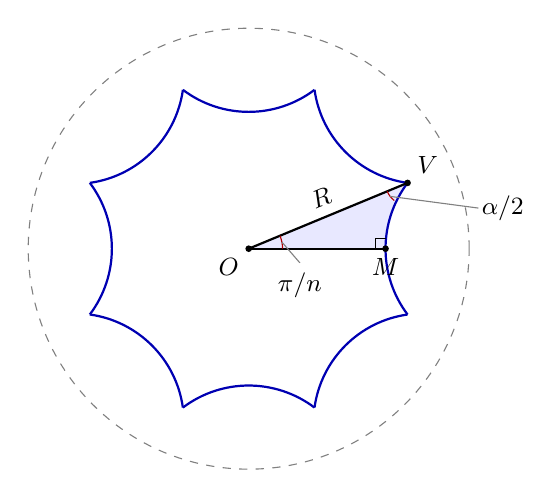
\begin{tikzpicture}[font=\small]
	\pgfmathsetmacro{\PlotRadius}{2.8}
	\pgfmathsetmacro{\VertexRadius}{.78}
	\pgfmathsetmacro{\HalfAngle}{22.5}
	\pgfmathsetmacro{\CircleCenter}{(1+\VertexRadius^2)/(2*\VertexRadius*cos(\HalfAngle))}
	\pgfmathsetmacro{\CircleRadius}{sqrt(\CircleCenter^2-1)}
	\pgfmathsetmacro{\ArcAngle}{atan2(\VertexRadius*sin(\HalfAngle),\CircleCenter-\VertexRadius*cos(\HalfAngle))}
	\pgfmathsetmacro{\Midpoint}{\PlotRadius*(\CircleCenter-\CircleRadius)}
	\coordinate (O) at (0,0);
	\coordinate (M) at (\Midpoint,0);
	\coordinate (V) at ({\PlotRadius*\VertexRadius*cos(\HalfAngle)},{\PlotRadius*\VertexRadius*sin(\HalfAngle)});
	\fill[blue!9] (O)--(M) arc[start angle=180,end angle={180-\ArcAngle},radius={\PlotRadius*\CircleRadius}]--cycle;
	\draw[dashed,gray] (O) circle (\PlotRadius);
	\foreach \j in {0,...,7}{
		\pgfmathsetmacro{\MiddleAngle}{45*\j}
		\draw[thick,blue!70!black] ({\PlotRadius*\VertexRadius*cos(\MiddleAngle-\HalfAngle)},{\PlotRadius*\VertexRadius*sin(\MiddleAngle-\HalfAngle)}) arc[start angle={\MiddleAngle+180+\ArcAngle},end angle={\MiddleAngle+180-\ArcAngle},radius={\PlotRadius*\CircleRadius}];
	}
	\draw[thick] (O)--(M);
	\draw[thick] (O)--node[midway,above,sloped] {\(R\)}(V);
	\draw (\Midpoint-.13,0)--(\Midpoint-.13,.13)--(\Midpoint,.13);
	\draw[red!70!black] (.43,0) arc[start angle=0,end angle=\HalfAngle,radius=.43];
	\node[below] at (.65,-.18) {\(\pi/n\)};
	\draw[thin,gray] (.65,-.18)--({.43*cos(\HalfAngle/2)},{.43*sin(\HalfAngle/2)});
	\begin{scope}[shift={(V)}]
		\draw[red!70!black] ({.28*cos(180+\HalfAngle)},{.28*sin(180+\HalfAngle)}) arc[start angle={180+\HalfAngle},end angle={270-\ArcAngle},radius=.28];
		\draw[thin,gray] ({.28*cos((450+\HalfAngle-\ArcAngle)/2)},{.28*sin((450+\HalfAngle-\ArcAngle)/2)})--(.9,-.32);
		\node[right,fill=white,inner sep=1pt] at (.9,-.32) {\(\alpha/2\)};
	\end{scope}
	\foreach \p in {O,M,V}{\fill (\p) circle (1.2pt);}
	\node[below left] at (O) {\(O\)};
	\node[below] at (M) {\(M\)};
	\node[above right] at (V) {\(V\)};
\end{tikzpicture}

	\caption[正则双曲多边形的直角三角形]{圆盘模型中的正则八边形。中心 \(O\)、边中点 \(M\) 与顶点 \(V\) 构成直角三角形，\(OV=R\)，中心角为 \(\pi/n\)，顶点角为 \(\alpha/2\)。虚线圆周是理想边界；测地边向圆盘中心一侧弯曲。}
	\label{g1:fig:regular-hyperbolic-polygon}
\end{figure}

角条件在粘合时有直接含义。若若干多边形顶点被识别成一个点，它们围出的角必须合计 \(2\pi\)，才可能成为普通光滑曲面点；否则会留下圆锥型的角亏或角盈。上面的 \(4g\) 个角之和正是 \(2\pi\)，而边长相等允许按保向等距匹配有序端点。下一节还会逐项检查边两侧的光滑接合、顶点邻域以及整体商空间；这里的多边形构造提供了所需的具体长度与角度数据。

% !TeX root = ../../Book1.tex
% 纲要标题：### 10.2 离散群与曲面商
% 纲要位置：几何学计划纲要.md，第 515 行。
% 正文状态：初稿；尚未正式审核。

% 纲要内容开始
% 
% * 椭圆、抛物和双曲变换
% * 自由固有作用及基本区域
% * 基本多边形的边配对与粘合
% * 闭曲面、尖点与漏斗的模型
% 
% 纲要内容结束

\section{离散群与曲面商}
\label{g1:sec:1002}

双曲平面中每一点的局部几何都相同，但把不同的点按等距变换识别以后，可以得到有闭测地线的圆柱、面积有限的尖点端，乃至任意亏格不小于二的闭曲面。这里有两个不同的构造问题：给定一个等距变换群，商是否仍是光滑曲面；给定一张多边形和边配对，接缝及顶点附近的度量是否光滑。前一个问题由作用的自由性和固有性控制，后一个问题必须逐条检查边的等距配对和顶点周围的总角。

\subsection{椭圆、抛物和双曲变换}
\label{g1:subsec:1002:01}

在上半平面 \(\mathbb H=\{z=x+iy:y>0\}\) 上，度量为 \(g_{\mathbb H}=|\mathrm{d}z|^2/y^2\)。\cref{g1:thm:hyperbolic-isometry-group}已经说明，其保向等距变换恰为
\[
	z\longmapsto\frac{az+b}{cz+d},\qquad
	A=\begin{pmatrix}a&b\\c&d\end{pmatrix}\in\operatorname{SL}(2,\mathbb R),
\]
其中 \(A\) 与 \(-A\) 给出同一个变换，因此群为 \(\operatorname{PSL}(2,\mathbb R)\)。这些变换也作用于理想边界 \(\mathbb R\cup\{\infty\}\)；那里不是双曲平面的一部分，边界不动点与平面内不动点必须区别。

\begin{theorem}[保向等距变换的分类]\label{g1:thm:psl-element-classification}
	设 \(h\in\operatorname{PSL}(2,\mathbb R)\) 不是恒等变换，取代表矩阵 \(A\in\operatorname{SL}(2,\mathbb R)\)，记 \(\tau=(\operatorname{tr}A)^2\)。则有且仅有下列一种情形。
	\begin{enumerate}
		\item \(\tau<4\)：\(h\) 在 \(\mathbb H\) 中有唯一不动点，在理想边界没有不动点；移到圆盘模型并把该点移到原点后，\(h\) 为非恒等旋转 \(w\mapsto e^{i\theta}w\)。称 \(h\) 为\term[tuoyuanbianhuan]{椭圆变换}[elliptic isometry]。
		\item \(\tau=4\)：\(h\) 在 \(\mathbb H\) 中没有不动点，在理想边界有唯一不动点；经保向等距共轭后，\(h\) 为 \(z\mapsto z+1\) 或 \(z\mapsto z-1\)。称 \(h\) 为\term[paowubianhuan]{抛物变换}[parabolic isometry]。
		\item \(\tau>4\)：\(h\) 在 \(\mathbb H\) 中没有不动点，在理想边界有两个不同不动点；经保向等距共轭后，\(h\) 为 \(z\mapsto e^\ell z\)，其中 \(\ell>0\) 且
		\[
			|\operatorname{tr}A|=2\cosh(\ell/2).
		\]
		称 \(h\) 为\term[shuangqubianhuan]{双曲变换}[hyperbolic isometry]。
	\end{enumerate}
\end{theorem}
\begin{proof}
	更换代表 \(A\mapsto-A\) 不改变 \(\tau\)，共轭也不改变它。有限不动点满足
	\[
		cz^2+(d-a)z-b=0,
	\]
	其判别式为 \((a+d)^2-4(ad-bc)=\tau-4\)。若 \(c=0\)，还要把无穷远点计入；统一地说，理想边界不动点就是实矩阵 \(A\) 的实特征直线，所以判别式同样区分零个、一个和两个实不动点。

	若 \(\tau<4\)，两个非实根互为共轭，恰有一个在 \(\mathbb H\) 中。设它为 \(p=x+iy\)，变换 \(z\mapsto(z-x)/y\) 将其送到 \(i\)。一个实 Möbius 变换固定 \(i\) 当且仅当其代表可写成
	\[
		R_\theta=\begin{pmatrix}
			\cos(\theta/2)&\sin(\theta/2)\\
			-\sin(\theta/2)&\cos(\theta/2)
		\end{pmatrix}.
	\]
	用圆盘坐标 \(w=(z-i)/(z+i)\) 代入，所得变换为 \(w\mapsto e^{i\theta}w\)。非恒等性排除 \(\theta\equiv0\pmod{2\pi}\)，也给出平面内不动点的唯一性。

	若 \(\tau=4\)，非恒等性说明 \(A\ne\pm I\)，故只有一条实特征直线。将它送到 \(\infty\)，变换便写成 \(z\mapsto a^2z+ab\)，其中代表矩阵的对角元为 \(a,a^{-1}\)。迹平方等于四迫使 \(a=\pm1\)，于是它是非零平移 \(z\mapsto z+t\)。再用正缩放共轭，将 \(|t|\) 变成 \(1\)。正、负两个方向都保留在陈述中，因为保向共轭不能随意把这两个标准型混为同一个。

	若 \(\tau>4\)，将两个理想不动点送到 \(0,\infty\)，得到 \(z\mapsto\lambda z\)，其中 \(\lambda>0\) 且 \(\lambda\ne1\)。若 \(\lambda<1\)，再用 \(z\mapsto-1/z\) 交换两端，便可令 \(\lambda=e^\ell>1\)。代表矩阵可取 \(\operatorname{diag}(e^{\ell/2},e^{-\ell/2})\)，给出迹的公式。三个标准型的全部不动点均已列出，证明分类。
\end{proof}

迹平方判别的是三种类型，不是所有共轭参数。例如圆盘中旋转 \(\theta\) 与旋转 \(-\theta\) 具有相同的迹平方，但保向共轭还保留旋转方向。下一步要构造商时，更重要的是一个变换把点移动了多远。

\begin{definition}[平移长度]\label{g1:def:hyperbolic-translation-length}
	设 \(\mathbb H\) 为曲率 \(-1\) 的双曲平面，\(d_{\mathbb H}\) 为其长度距离，\(h:\mathbb H\to\mathbb H\) 为等距变换。它的\term[pingyichangdu]{平移长度}[translation length]定义为
	\[
		L(h)=\inf_{p\in\mathbb H}d_{\mathbb H}(p,hp).
	\]
\end{definition}

对椭圆变换，\(L(h)=0\)，且在唯一内点不动点处达到。对抛物变换 \(z\mapsto z+t\)，\cref{g1:thm:hyperbolic-distance-geodesics}中的距离公式给出
\[
	\cosh d_{\mathbb H}(z,z+t)=1+\frac{t^2}{2y^2},
\]
所以 \(L(h)=0\)，但没有任何平面内点达到这个下确界。对双曲标准型，距离公式则给出
\begin{equation}\label{g1:eq:hyperbolic-displacement}
	\cosh d_{\mathbb H}(z,e^\ell z)
	=\cosh\ell+2\sinh^2(\ell/2)\frac{x^2}{y^2}.
\end{equation}
因此 \(L(h)=\ell\)，恰在虚轴上达到。一般双曲变换的两个理想不动点之间的测地线称为它的\term[zhou]{轴}[axis]；沿轴的作用就是长度为 \(\ell\) 的平移。下确界是否达到，已经把抛物与双曲两种无内点不动点的行为区别开来。

\subsection{自由固有作用及基本区域}
\label{g1:subsec:1002:02}

为了使商附近仍是一张普通小圆盘，需要排除两种障碍：一个群元素固定该点，或者无限多个不同群元素在附近反复堆积。前者由自由性排除，后者由下面的紧集条件控制。

\begin{definition}[离散子群与固有作用]\label{g1:def:discrete-proper-isometric-action}
	给 \(\operatorname{PSL}(2,\mathbb R)\) 赋予矩阵群模去 \(\{\pm I\}\) 的拓扑。若子群 \(\Gamma\) 有一个单位元邻域只包含其单位元，就称它为\term[lisanziqun]{离散子群}[discrete subgroup]。对群在 \(\mathbb H\) 上的作用，若 \(\gamma p=p\) 蕴含 \(\gamma=1\)，就称它为\term[ziyouzuoyong]{自由作用}[free action]；若对每个紧集 \(K\subset\mathbb H\)，集合
	\[
		\{\gamma\in\Gamma:\gamma K\cap K\ne\varnothing\}
	\]
	有限，就称它为\term[guyouzuoyong]{固有作用}[proper action]。
\end{definition}

这里把 \(\Gamma\) 当作离散群，使用的是适合离散作用的紧集定义。第五章\cref{g1:def:properly-discontinuous-covering}中的“适当不连续”还要求每点都有与所有非平凡平移不交的小邻域，因而已经包含自由性。本节的固有性允许有限稳定子；要恢复第五章的条件，需要同时假设自由。

\begin{proposition}[离散性与固有性]\label{g1:prop:discrete-hyperbolic-action}
	子群 \(\Gamma\subset\operatorname{PSL}(2,\mathbb R)\) 离散，当且仅当其在 \(\mathbb H\) 上的作用固有。离散子群中的椭圆元素都有有限阶；其作用自由，当且仅当它没有非单位有限阶元素。
\end{proposition}
\begin{proof}
	先说明离散子群与任意紧的群元素集合只有有限交。若紧集内有无限个不同元素 \(\gamma_n\)，由矩阵空间的紧性可取收敛子列；于是不同的 \(\gamma_n^{-1}\gamma_m\) 可以任意接近单位元，与单位元孤立矛盾。这里并未假定子群先验闭；同一个论证也说明其在矩阵群中的任何收敛序列最终恒定，所以它确实闭。

	给 \(p=x+iy\) 选连续依赖于 \(p\) 的等距变换
	\[
		u_p(z)=yz+x,\qquad
		u_p=\left[\begin{pmatrix}\sqrt y&x/\sqrt y\\0&1/\sqrt y\end{pmatrix}\right],
	\]
	它将 \(i\) 送到 \(p\)。若 \(h p=q\)，则 \(u_q^{-1}hu_p\) 固定 \(i\)，故属于前面写出的旋转群 \(\{R_\theta\}\)，这是一个紧群。若 \(p,q\in K\)，那么 \(h\) 位于紧集
	\[
		\{u_qR_\theta u_p^{-1}:p,q\in K,\ 0\le\theta\le2\pi\}
	\]
	之中。离散子群与该紧集只有有限交，故作用固有。反过来，若有不同的 \(\gamma_n\) 趋于单位元，则 \(\gamma_ni\to i\)；包含这些点和 \(i\) 的一个小紧邻域 \(K\) 将满足 \(\gamma_nK\cap K\ne\varnothing\)，与固有性矛盾。

	椭圆元素的所有幂都位于一个共轭旋转群中，后者紧，所以离散性迫使其幂只有有限多个，即该元素为有限阶。分类定理表明，非恒等抛物或双曲变换都有无限阶。因此没有非单位有限阶元素等价于没有椭圆元素，又等价于没有平面内不动点，即作用自由。
\end{proof}

例如绕同一点旋转 \(2\pi/m\) 生成的有限群离散且作用固有，却不自由；这个点在商中有锥角 \(2\pi/m\)。绕同一点旋转一个与 \(2\pi\) 之比为无理数的角所生成的群则不离散，因为它有无限多个幂落在同一个紧旋转群中。离散性不会自动排除所有不动点。

\begin{theorem}[自由固有等距作用的商]\label{g1:thm:hyperbolic-quotient}
	设 \(\Gamma\subset\operatorname{PSL}(2,\mathbb R)\) 自由且固有地作用于 \(\mathbb H\)。则轨道商 \(M=\mathbb H/\Gamma\) 是 Hausdorff、第二可数的可定向光滑曲面，且有唯一度量使投影 \(q:\mathbb H\to M\) 为局部等距。该度量曲率恒为 \(-1\)，长度距离完备；\(q\) 是万有覆盖，覆盖变换群恰为 \(\Gamma\)。
\end{theorem}
\begin{proof}
	固定 \(p\in\mathbb H\)，取包含它的紧邻域 \(K\)。只有有限个 \(\gamma\) 满足 \(\gamma K\cap K\ne\varnothing\)。自由性给出 \(\gamma p\ne p\)；对有限个这样的非单位元素，同时缩小 \(p\) 的邻域 \(U\)，即可使 \(\gamma U\cap U=\varnothing\)。其余元素由 \(U\subset K\) 已经排除。因此第五章的强适当不连续条件成立。\cref{g1:prop:action-quotient-cover}的证明给出 \(q\) 为开映射，以及
	\[
		q^{-1}(q(U))=\bigsqcup_{\gamma\in\Gamma}\gamma U,
	\]
	每张片都同胚映到 \(q(U)\)。上半平面凸且可缩，特别是单连通；该命题还说明这是万有覆盖，覆盖变换群正是 \(\Gamma\)。

	仍须核验商的分离性。若 \(p,r\) 不在同一轨道，取它们的紧邻域之并 \(K\)。可能把第一个邻域送到第二个的群元素只有有限个；又因 \(\gamma p\ne r\)，可以同时缩小成 \(U\ni p,V\ni r\)，使所有 \(\gamma U\) 都不交 \(V\)。于是 \(q(U),q(V)\) 是不交开邻域，故商 Hausdorff。\(\mathbb H\) 的可数开基经开映射 \(q\) 取像，仍是商的可数开基，得到第二可数性。

	用 \(q|_U\) 的逆把 \(q(U)\) 当作上半平面小片。两个这样的图在每个足够小的交叠部分上相差唯一一个 \(\gamma\in\Gamma\)，因而转换是光滑保向等距。各片的度量便相容地下降，唯一性也由局部等距要求决定；局部曲率保持为 \(-1\)。

	最后证明完备性，而不由“局部等距”直接推出。距离公式说明 \(d_{\mathbb H}(i,x+iy)\le R\) 等价于
	\[
		x^2+(y-\cosh R)^2\le\sinh^2R.
	\]
	这个 Euclid 闭圆盘的最低高度为 \(e^{-R}>0\)，所以双曲闭球紧。固有性于是保证轨道与每个闭有界球只有有限交，故
	\begin{equation}\label{g1:eq:hyperbolic-quotient-distance}
		d_M(qx,qy)=\min_{\gamma\in\Gamma}d_{\mathbb H}(x,\gamma y).
	\end{equation}
	具体地，右端的最小值存在；不同轨道之间它为正，三角不等式由等距不变性得到。投影任意连接 \(x\) 与 \(\gamma y\) 的测地段，说明商长度距离不超过它。反过来，商中的每条分片光滑连接曲线从 \(x\) 提升后终于某个 \(\gamma y\)，提升保持长度，故其长度至少为右端。这样就证明了等式。

	对 \(M\) 中任一 Cauchy 序列，取子列 \(p_n\)，使 \(d_M(p_n,p_{n+1})<2^{-n}\)。从任意提升 \(x_1\) 开始，逐次用\eqref{g1:eq:hyperbolic-quotient-distance}选择提升 \(x_{n+1}\)，满足 \(d_{\mathbb H}(x_n,x_{n+1})<2^{-n}\)。这些提升构成 Cauchy 序列，在完备的 \(\mathbb H\) 中收敛；其投影给出 \(p_n\) 的极限。原序列因 Cauchy 性也收敛，故商完备。
\end{proof}

上述证明把拓扑和度量的责任分开了：局部不交邻域给出覆盖，固有性还保证不同轨道能被分离，而等距性才使局部度量在商上相容。

\begin{definition}[Dirichlet 区域]\label{g1:def:dirichlet-domain}
	设 \(\Gamma\subset\operatorname{PSL}(2,\mathbb R)\) 的作用自由且固有，固定 \(p\in\mathbb H\)。集合
	\[
		D_p=\{x\in\mathbb H:d_{\mathbb H}(x,p)\le d_{\mathbb H}(x,\gamma p)\ \text{对所有 }\gamma\in\Gamma\}
	\]
	称为以 \(p\) 为中心的\term[Dirichletquyu]{Dirichlet 区域}[Dirichlet domain]。它把“离哪一个轨道点最近”转化成一组半平面条件。\footnote{Johann Peter Gustav Lejeune Dirichlet（1805--1859），德国数学家，对数论、Fourier 级数与势理论作出重要贡献。}
\end{definition}

\begin{proposition}[Dirichlet 区域的铺盖]\label{g1:prop:dirichlet-domain}
	设 \(\Gamma\subseteq\operatorname{PSL}(2,\mathbb R)\) 以标准双曲等距自由且固有地作用于 \(\mathbb H\)，\(p\in\mathbb H\)，\(d\) 为双曲距离。令 \(D_p=\{x\in\mathbb H:d(x,p)\le d(x,\gamma p)\text{ 对所有 }\gamma\in\Gamma\}\)。则 \(D_p\) 是有非空内部的闭测地凸集，所有 \(\gamma D_p\) 覆盖 \(\mathbb H\)，不同平移的内部不交；这些平移局部有限。\(D_p\) 在每个有界部分由有限条测地边界限制。若 \(\mathbb H/\Gamma\) 紧，则 \(D_p\) 是紧的有限边测地多边形。
\end{proposition}
\begin{proof}
	两个不同点 \(p,q\) 的等距轨迹是一条测地线，\(d(x,p)\le d(x,q)\) 选出包含 \(p\) 的闭半平面。在双曲面模型中可以直接看出这一点：距离公式把等距条件写成 Lorentz 内积的线性等式 \(\langle X,P-Q\rangle_L=0\)，而 \(P-Q\) 为空间样向量；该平面截双曲面得到测地线。每一侧测地凸，因为长为 \(L>0\) 的测地段在双曲面上的表达是
	\[
		X(t)=\frac{\sinh((1-t)L)}{\sinh L}X(0)
		+\frac{\sinh(tL)}{\sinh L}X(1),\qquad 0\le t\le1,
	\]
	两系数均非负，保持同侧的线性不等式。因此 \(D_p\) 是闭测地凸集。固有性和自由性给出 \(\inf_{\gamma\ne1}d(p,\gamma p)>0\)，取该下界一半以内的小球，就包含在 \(D_p\) 的内部。

	对任意 \(x\)，轨道 \(\Gamma p\) 中有一个距 \(x\) 最近的点，存在性与商距离的最小值相同。若最近点为 \(\gamma p\)，则 \(\gamma^{-1}x\in D_p\)，所以各平移覆盖。若 \(x\) 同时位于 \(\gamma D_p\) 和 \(\eta D_p\) 的内部，且 \(\gamma\ne\eta\)，第一个内部条件给出 \(d(x,\gamma p)<d(x,\eta p)\)，第二个给出反向严格不等式，矛盾。严格性来自等距轨迹是一条边界测地线，不能包含内点。

	若 \(x\in\overline B(p,R)\cap\gamma D_p\)，最近点条件说明 \(d(x,\gamma p)\le d(x,p)\le R\)，于是 \(d(p,\gamma p)\le2R\)。这样的 \(\gamma\) 只有有限个，得到平移的局部有限性。同样，在 \(B(p,R)\) 内能限制 \(D_p\) 的半平面只可能来自 \(d(p,\gamma p)\le2R\) 的元素，因为更远的轨道点在此球中总比 \(p\) 远。因此每个有界部分只需有限条边界。

	若商紧，递增开集 \(q(B(p,R))\) 覆盖它，紧性给出某个 \(R\) 已经覆盖全商。每个 \(x\in D_p\) 都与 \(B(p,R)\) 中某点等价，故它距某个轨道点小于 \(R\)，最近点条件进一步给出 \(d(x,p)<R\)。于是 \(D_p\) 闭且有界，从而紧；它全部位于一个稍大的球内，所需边界只有有限条，得到有限测地多边形。
\end{proof}

满足覆盖且内部不重叠的这样的闭区域称为群作用的\term[jibenquyu]{基本区域}[fundamental domain]。边界上可以有多个代表，必须按群元素识别，不能要求每条轨道与闭区域恰交一次。非紧商的 Dirichlet 区域也未必只有有限条边，上命题只保证有界范围内的有限性。

\subsection{基本多边形的边配对与粘合}
\label{g1:subsec:1002:03}

反过来，可以先画一张双曲多边形，再沿成对的边接合。第六章\cref{g1:thm:surface-polygon}及\cref{g1:prop:orientable-standard-word}解释了边字如何记录拓扑粘合；现在还要使这些粘合保留度量。边内点的邻域由两张半圆盘组成，顶点的邻域则由若干个角扇组成，两处需要不同的检查。

\begin{proposition}[双曲多边形的光滑粘合]\label{g1:prop:hyperbolic-polygon-gluing}
	设 \(P\subset\mathbb H\) 是紧凸测地多边形，将不同的边两两配对，每对等长，并用保向双曲等距变换按相反的边界行进方向识别。对每个顶点等价类，将其各角的一条小圆弧按边配对接起；假设所得空间是一条圆周，且该类内的角度总和为 \(2\pi\)。则商 \(P/{\sim}\) 是紧、可定向、无边界的光滑曲面，\(P\) 的双曲度量在其上光滑粘合，曲率恒为 \(-1\)。
\end{proposition}
\begin{proof}
	等长测地边的端点可以按要求配对：先用\cref{g1:prop:model-isometry-data}将一条边的起点及单位切向量送到另一条边的终点及反向单位切向量；测地线的初值唯一性使整条等长边随之对应。保向性保证原来的内侧被送到另一条边的外侧，因此两侧窄半盘在识别后确实拼成一个双曲小圆盘，度量在接缝处光滑。

	这里的商也是 Hausdorff。等价关系在 \(P\times P\) 中由对角线、有限个闭边配对映射的图以及有限个顶点等价对组成，故为闭集。若 \(C\subset P\) 闭，它的饱和集是此闭关系与 \(C\times P\) 的交在第二因子的投影，因紧性而闭。两个不同等价类是 \(P\) 中不交的有限集，取不交开邻域 \(U,V\) 包含它们；从 \(U\) 中去掉所有与 \(P\setminus U\) 等价的点，得到包含原等价类的饱和开集，\(V\) 同理。两者下降为商中不交开邻域。商紧性来自 \(P\) 的紧性。

	在一个顶点类处，将各原顶点附近截成同样小半径的角扇。边等距保留距相应顶点的距离，故各扇可以用同一个径向变量 \(r\) 粘合。双曲面极坐标
	\[
		(r,\theta)\longmapsto(\cosh r,\sinh r\cos\theta,\sinh r\sin\theta)
	\]
	直接给出度量 \(\mathrm{d}r^2+\sinh^2r\,\mathrm{d}\theta^2\)。把各扇按圆弧连接的次序排好，角变量逐段累计；小圆弧接成一条圆周意味着绕行只形成一个扇环，总角 \(2\pi\) 则使这个扇环恰好拼成普通双曲小圆盘。末缝处 \(\theta=0\) 与 \(2\pi\) 的极坐标映射以及所有导数相容，中心也由上述双曲面坐标给出通常的光滑结构。因此顶点没有锥形奇点。

	面内、边内和顶点处的这些局部图在交叠处相差双曲等距变换，形成相容的光滑图册和度量。各边都已配对，故没有边界；配对反转边界行进方向而保持环境定向，所以局部定向也相容。紧性允许从局部图取有限覆盖，每张图有可数基，故商第二可数。这就得到所述光滑度量曲面。
\end{proof}

顶点附近的小圆弧拼成的圆周常称为该顶点的\term[lianjie]{链接}[link]。链接控制局部邻域是不是一张盘，总角则控制这张盘上的度量是否光滑。若链接仍是一条圆周但总角为 \(\Theta\ne2\pi\)，小半径圆周的长度就是 \(\Theta\sinh r\)，除以半径后趋于 \(\Theta\)，不能是光滑曲面中应有的 \(2\pi\)。因此检查边长相等还不够。

\ProseParagraphBreak

这一命题构造的是有限多边形的度量商。若另把边配对变换放进 \(\operatorname{PSL}(2,\mathbb R)\) 并取它们生成的群，还需要证明其离散性及原多边形的平移是否铺盖整个平面；这些整体结论不是一句“角和为 \(2\pi\)”就能直接替代的。下一节将用展开映射说明完备模型结构的整体实现。

\begin{theorem}[闭双曲曲面的多边形构造]\label{g1:thm:closed-hyperbolic-polygon}
	设 \(g\ge2\) 为整数，\(\Sigma_{g,0}\) 为可定向亏格 \(g\) 的闭曲面。存在一张与 \(\Sigma_{g,0}\) 同胚的紧光滑曲面，带曲率恒为 \(-1\) 的度量。它可以由曲率 \(-1\) 双曲平面中一个内角均为 \(\pi/(2g)\) 的凸正则测地 \(4g\) 边形按边字
	\[
		a_1b_1a_1^{-1}b_1^{-1}\cdots a_gb_ga_g^{-1}b_g^{-1}
	\]
	将同字母边按相反边界方向，用保向双曲等距两两配对得到，面积为 \(4\pi(g-1)\)。
\end{theorem}
\begin{proof}
	\cref{g1:prop:regular-hyperbolic-polygons}保证：给定 \(n\ge3\) 及 \(0<\alpha<(n-2)\pi/n\)，存在内角为 \(\alpha\) 的正则双曲 \(n\) 边形。对 \(n=4g\)、\(\alpha=\pi/(2g)\)，所需严格不等式恰由 \(g\ge2\) 保证。所有边等长，故按上命题可实施指定的等距配对。

	还要检查顶点，不能只因共有 \(4g\) 个角就默认它们拼在同一点。依次记顶点为 \(v_0,\ldots,v_{4g-1}\)，第 \(j\) 条边从 \(v_j\) 指向 \(v_{j+1}\)，下标模 \(4g\)。在第 \(k\) 个四边块中，\(a\) 配对给出
	\[
		v_{4k}\sim v_{4k+3},\qquad v_{4k+1}\sim v_{4k+2},
	\]
	\(b\) 配对给出 \(v_{4k+1}\sim v_{4k+4}\) 及 \(v_{4k+2}\sim v_{4k+3}\)。这些关系把该块的五个连续端点连在一起，因而所有顶点属于一个等价类。

	再从一个角的小圆弧穿过配对边进入下一个角，所得链接的后继顺序为
	\[
		4k+1\longmapsto4k+2\longmapsto4k+3\longmapsto4k
		\longmapsto4(k-1)+1
	\]
	（所有下标模 \(4g\)）。它先走过一个四边块的四个角，再进入前一个四边块，最终恰走过全部 \(4g\) 个角一次才返回，故链接是单一圆周。总角为 \(4g\cdot\pi/(2g)=2\pi\)，上命题给出光滑双曲度量。

	这个边字的拓扑类型由\cref{g1:prop:orientable-standard-word}中标准字与手柄连通和的对应给出，正是 \(\Sigma_{g,0}\)。最后，\cref{g1:prop:geodesic-polygon-area}给出
	\[
		\operatorname{Area}(P)=(4g-2)\pi-4g\frac{\pi}{2g}=4\pi(g-1).
	\]
	边及顶点的识别不改变面积，故商也有这个面积。
\end{proof}

对 \(g=1\)，所需四边形的四个角都为 \(\pi/2\)，角和达到平面四边形的角和 \(2\pi\)，双曲面积公式将给出零面积，所以这种非退化双曲四边形不存在。这与第九章 Gauss--Bonnet 排除闭环面上的负常曲率度量相符。

\subsection{闭曲面、尖点与漏斗的模型}
\label{g1:subsec:1002:04}

刚才得到的闭曲面紧，长度距离因而完备：局部双曲图中的度量在小闭片上与 Euclid 度量双边可比，长度距离给出原拓扑；任一 Cauchy 序列都有由紧性提供的收敛子列，进而整个序列收敛。它们的面积有限，但非紧曲面也可能有有限面积的端部。两种最简单的非紧端部来自抛物和双曲循环群。

\begin{example}[尖点]\label{g1:exm:hyperbolic-cusp}
	令 \(T(z)=z+1\)。群 \(\langle T\rangle\) 离散且自由，整个商 \(\mathbb H/\langle T\rangle\) 是完备双曲圆柱。固定 \(Y>0\)，取其中由 \(y\ge Y\) 给出的端部
	\[
		C_Y=\{y\ge Y\}/\langle T\rangle.
	\]
	这是\term[jiandian]{尖点}[cusp]的标准模型。其一条基本条带为 \(0\le x\le1,y\ge Y\)，两条竖边配对。令 \(r=\log(y/Y)\)，则
	\begin{equation}\label{g1:eq:hyperbolic-cusp-metric}
		g=\mathrm{d}r^2+Y^{-2}e^{-2r}\,\mathrm{d}x^2,
		\qquad r\ge0,\quad x\in\mathbb R/\mathbb Z.
	\end{equation}
	截圈 \(r=R\) 的长度为 \(Y^{-1}e^{-R}\)，向尖端越来越短；但是任何向 \(r\to\infty\) 行进的曲线长度至少为其 \(r\) 的总变化，所以尖端处在无限距离处。另一方面，
	\[
		\operatorname{Area}(C_Y)=\int_0^1\int_Y^\infty\frac{\mathrm{d}y\,\mathrm{d}x}{y^2}=\frac1Y.
	\]
	因此无限距离与有限面积可以同时出现。这里 \(C_Y\) 是带截口的端部；整个完备平移商还包含 \(0<y<Y\) 的另一端，其面积无限。不能把有限面积端部和整个圆柱的面积混为一谈。
\end{example}

\begin{proposition}[双曲圆柱的 Fermi 坐标]\label{g1:prop:hyperbolic-cylinder-fermi}
	设 \(\ell>0\)，令 \(H(z)=e^\ell z\)。完备双曲圆柱 \(\mathbb H/\langle H\rangle\) 有全局坐标
	\[
		r\in\mathbb R,\qquad t\in\mathbb R/\ell\mathbb Z,
		\qquad g=\mathrm{d}r^2+\cosh^2r\,\mathrm{d}t^2.
	\]
	\(r=0\) 是长度 \(\ell\) 的闭测地线，\(|r|\) 是距它的距离；\(r\ge0\) 与 \(r\le0\) 分别给出一个\term[loudou]{漏斗}[funnel]，各漏斗的面积无限。
\end{proposition}
\begin{proof}
	在 \(\mathbb H\) 中直接置
	\[
		x=e^t\tanh r,\qquad y=e^t\operatorname{sech}r.
	\]
	其逆为 \(t=\log\sqrt{x^2+y^2}\)、\(r=\operatorname{arsinh}(x/y)\)，所以这是全局坐标。求微分后交叉项抵消，得到
	\[
		\mathrm{d}x^2+\mathrm{d}y^2
		=e^{2t}\bigl(\mathrm{d}t^2+\operatorname{sech}^2r\,\mathrm{d}r^2\bigr).
	\]
	除以 \(y^2=e^{2t}\operatorname{sech}^2r\) 即得所述度量。缩放 \(z\mapsto e^\ell z\) 恰对应 \(t\mapsto t+\ell\)，故坐标下降到圆柱。群的离散性与自由性由缩放标准型直接得到，完备性由\cref{g1:thm:hyperbolic-quotient}保证。

	\(r=0\) 是虚轴的像，因而为闭测地线，其长度就是 \(t\) 的周期 \(\ell\)。任一从 \(r\) 到零的曲线长度至少为 \(|r|\)，固定 \(t\) 的径向段达到它，因此 \(|r|\) 是到轴的距离。在 \(r\ge0\) 一侧，截圈长度为 \(\ell\cosh r\)，面积元为 \(\cosh r\,\mathrm{d}r\,\mathrm{d}t\)，所以
	\[
		\operatorname{Area}(0\le r\le R)=\ell\sinh R\longrightarrow\infty.
	\]
	另一侧由 \(r\mapsto-r\) 对称得到相同结论。
\end{proof}

上述以测地线为基线、以法向距离 \(r\) 为横坐标的坐标称为\term[Fermizuobiao]{Fermi 坐标}[Fermi coordinates]。\footnote{Enrico Fermi（1901--1954），意大利出生的美国物理学家，研究量子理论、统计力学与核物理。}尖点截圈的长度指数衰减，漏斗截圈的长度按 \(\cosh r\) 增长，这是两种端部面积行为不同的直接原因。\cref{g1:fig:cusp-funnel-domains}把两个循环群的基本区域画在同一个上半平面模型中。

% !TeX root = ../Book1.tex
\begin{figure}[htbp]
	\centering
	\begin{tikzpicture}[scale=0.95,font=\small]
		\begin{scope}[xshift=-3.1cm]
			\fill[GeometryBlueLight] (0,0.9) rectangle (1.7,3.1);
			\draw[->] (-0.7,0)--(2.5,0) node[right] {\(x\)};
			\draw[GeometryBlue,thick] (0,0.35)--(0,3.25);
			\draw[GeometryBlue,thick] (1.7,0.35)--(1.7,3.25);
			\draw[GeometryBlue,dashed] (-0.4,0.9)--(2.1,0.9);
			\node[left] at (-0.4,0.9) {\(y=Y\)};
			\draw[->,GeometryBlue] (0,1.5)--(1.7,1.5) node[midway,above] {\(z\mapsto z+1\)};
			\draw[->,GeometryBlue] (0.85,2.2)--(0.85,3.2);
			\node[above] at (0.85,3.2) {尖端 \(y\to\infty\)};
			\node[below] at (0,0) {\(0\)};
			\node[below] at (1.7,0) {\(1\)};
			\node[align=center] at (0.85,-0.85) {平移商的尖点端\\竖边配对，阴影部分面积有限};
		\end{scope}
		\begin{scope}[xshift=3.7cm]
			\fill[GeometryBlueLight] (2.1,0) arc (0:180:2.1)--(-1.05,0) arc (180:0:1.05)--cycle;
			\draw[->] (-2.5,0)--(2.5,0) node[right] {\(x\)};
			\draw[GeometryBlue,thick] (2.1,0) arc (0:180:2.1);
			\draw[GeometryBlue,thick] (1.05,0) arc (0:180:1.05);
			\draw[GeometryGray,dashed] (0,0)--(0,2.7);
			\draw[GeometryBlue,very thick] (0,1.05)--(0,2.1);
			\node[right] at (0.06,1.6) {轴};
			\draw[->,GeometryBlue] (140:1.05)--(140:2.1);
			\node[above,align=center] at (-1.15,2.4) {\(z\mapsto e^\ell z\)};
			\node at (-1.5,0.45) {\(r<0\)};
			\node at (1.5,0.45) {\(r>0\)};
			\node[align=center] at (0,-0.85) {缩放商的基本区域\\两条半圆配对，轴两侧为漏斗};
		\end{scope}
	\end{tikzpicture}
	\caption[尖点与漏斗的基本区域]{左图截取 \(0\le x\le1,y\ge Y\)，仅表示平移商中的尖点端；右图取 \(1\le|z|\le e^\ell\)，表示整个缩放圆柱的一个基本区域。右图以半径比 \(2\) 示意，粗轴段配对后成为闭测地线。图中的 Euclid 大小不表示双曲长度。}
	\label{g1:fig:cusp-funnel-domains}
\end{figure}


闭曲面、尖点端和漏斗都具有相同的局部曲率 \(-1\)，它们的紧性、面积和环路长度却不同。模型与粘合给出了这些具体度量；若只知道一张抽象曲面处处局部等距于双曲平面，还不能省略展开及单值的论证就把它写成一个全局商。下一节将把这一环节独立证明。

% !TeX root = ../../Book1.tex
% 纲要标题：### 10.3 局部齐性结构及其单值
% 纲要位置：几何学计划纲要.md，第 522 行。
% 正文状态：初稿；尚未正式审核。

% 纲要内容开始
% 
% * 几何图册与过渡群
% * 展开映射的构造
% * 单值表示及等变性
% * 完备性与模型商的关系
% 
% ---
% 
% 纲要内容结束

\section{局部齐性结构及其单值}
\label{g1:sec:1003}

把一张平纸卷成圆柱，每一小片仍可摊回平面，但沿圆柱绕一圈以后，展开的位置会相差一个平移。这个差别不来自小片的曲率，而来自不同小片怎样拼接。前一节从模型中的群作用构造曲面，本节反过来从曲面上的局部模型出发，追踪一张图沿道路延续时如何变化。所得展开映射与单值表示将说明：什么时候局部模型确实能够拼成整个模型的商，什么时候只能得到一个不完备的局部结构。

\subsection{几何图册与过渡群}
\label{g1:subsec:1003:01}

本节的曲面均为非空、连通、无边界的 Hausdorff、第二可数曲面，沿用\cref{g1:def:topological-surface}的分离与可数条件。无边界的要求有实际作用：模型取整个 \(S^2,\mathbb R^2,\mathbb H^2\) 的开集，半圆盘边缘不在这类图册中。曲面局部道路连通，连通性因而保证道路连通；坐标小圆盘又保证局部单连通，能够使用第五章的万有覆盖。

\ProseParagraphBreak

先取连通光滑模型曲面 \(X\)，以及通过光滑微分同胚作用在 \(X\) 上的群 \(G\)。若只有单位元在整个 \(X\) 上逐点不动，就称该作用有效。本节还要求一个更强的局部确定性质：
\begin{equation}
	\label{g1:eq:model-local-determination}
	g|_O=h|_O,\quad O\subset X\text{ 非空开}
	\quad\Longrightarrow\quad g=h.
\end{equation}
有效性本身不足以推出这一点。一般光滑微分同胚可以在一个开集上为恒等，在远处才发生变化；此时从局部换图无法唯一恢复群元素。对于连通模型的等距群，\cref{g1:prop:isometry-initial-data}说明等距由一点及该点的导数决定，故满足\eqref{g1:eq:model-local-determination}。通常还要求 \(G\) 在 \(X\) 上传递，表示模型各点没有区别；下述延续构造实际使用的是局部确定性质。

\begin{definition}
	\label{g1:def:geometry-atlas}
	设 \(X\) 为连通光滑曲面，\(G\le\operatorname{Diff}(X)\)，并满足局部确定性：若 \(g,h\in G\) 在 \(X\) 的某个非空开集上一致，则 \(g=h\)。设 \(M\) 为无边界拓扑曲面，\(\{U_i\}\) 为它的开覆盖。\(M\) 的一个\term[jihetuce]{几何图册}[geometric atlas]，或 \((G,X)\) 图册，是覆盖 \(M\) 的图
	\[
		\varphi_i:U_i\longrightarrow\varphi_i(U_i)\subset X,
	\]
	其中各 \(\varphi_i\) 为到开集的同胚，而且在任意交叠 \(U_i\cap U_j\) 的每个连通分支 \(C\) 上，存在 \(g_{ij,C}\in G\)，使
	\[
		\varphi_i|_C=g_{ij,C}\circ\varphi_j|_C.
	\]
	两个图册若其并仍满足此条件，就称为相容。一个相容图册类称为 \(M\) 的\term[jubuqixingjiegou]{局部齐性结构}[locally homogeneous structure]或 \((G,X)\) 结构。
\end{definition}

这些图自动给出光滑结构，因为换图映射是光滑微分同胚的限制。交叠处的群元素由\eqref{g1:eq:model-local-determination}唯一确定；在三图的共同小邻域中，
\[
	g_{ik}=g_{ij}g_{jk}.
\]
这里群乘法是函数复合：\((gh)(x)=g(h(x))\)。只在每个交叠分支上指定元素，是为了允许交叠不连通；没有理由要求几个分支使用同一个元素。

\ProseParagraphBreak

若 \(X\) 带度量 \(g_X\)、\(G\le\operatorname{Isom}(X)\)，各片上的 \(\varphi_i^*g_X\) 在交叠处一致，故定义了 \(M\) 上的光滑度量。这是一个具体的粘合验证：\(g_{ij}\) 保持 \(g_X\)，所以
\[
	\varphi_i^*g_X=\varphi_j^*(g_{ij}^*g_X)=\varphi_j^*g_X.
\]
由此得到的曲面每点附近都与模型等距。若过渡群包含非等距变换，例如平面的伸缩，图册仍有意义，却不能用这个公式粘合 Euclid 度量。

常曲率度量是否真的给出这种图册，也需要一个桥梁。这个问题只涉及小邻域，可以直接使用第九章已经建立的测地极坐标。

\begin{proposition}[常曲率的局部模型]
	\label{g1:prop:constant-curvature-local-model}
	设 \(M\) 是无边界光滑度量曲面，Gauss 曲率恒为 \(\kappa\in\{1,0,-1\}\)。则每点附近分别局部等距于单位球面、Euclid 平面或曲率为 \(-1\) 的双曲平面。这些局部等距给出 \((\operatorname{Isom}(X),X)\) 图册；若 \(M\) 已定向，可将过渡群限制为保向等距群。
\end{proposition}
\begin{proof}
	固定 \(p\in M\)。由\cref{g1:prop:normal-neighborhood,g1:lem:gauss-lemma}，中心之外的测地极坐标具有度量
	\[
		\mathrm{d}r^2+a(r,\theta)^2\,\mathrm{d}\theta^2,\qquad a>0.
	\]
	局部取与 \((\partial_r,\partial_\theta)\) 一致的定向。令 \(e_1=\partial_r\)、\(e_2=a^{-1}\partial_\theta\)。度量的 Christoffel 公式给出 \(\nabla_{\partial_r}e_1=0\)、\(\nabla_{\partial_\theta}e_1=a_r e_2\)，所以本书约定的联络形式为 \(\omega=a_r\,\mathrm{d}\theta\)。由\cref{g1:prop:connection-curvature-form}，
	\[
		a_{rr}\,\mathrm{d}r\wedge\mathrm{d}\theta
		=\mathrm{d}\omega=-K a\,\mathrm{d}r\wedge\mathrm{d}\theta,
		\qquad a_{rr}+\kappa a=0.
	\]

	中心处的初值不能只从极坐标公式形式地代入。取 \(\mathrm{T}_pM\) 中的单位向量 \(e(\theta)=(\cos\theta,\sin\theta)\)。第九章的构造实际给出
	\[
		a(r,\theta)=r\,b(r,\theta),\qquad
		b(r,\theta)=\left|\mathrm{d}(\exp_p)_{re(\theta)}(e'(\theta))\right|.
	\]
	指数映射在零附近光滑，且其零点微分为恒等；因而被取范数的向量在零附近不为零，\(b\) 对 \(r,\theta\) 光滑且 \(b(0,\theta)=1\)。所以 \(a\) 从 \(r\ge0\) 一侧光滑延到零，并满足 \(a(0,\theta)=0\)、\(a_r(0,\theta)=1\)。由\cref{g1:lem:smooth-ode-flow}所含的一阶系统唯一性，固定 \(\theta\) 后该标量方程的解只能是
	\[
		a(r,\theta)=S_\kappa(r),\qquad
		S_1(r)=\sin r,\quad S_0(r)=r,\quad S_{-1}(r)=\sinh r.
	\]
	这些函数直接满足方程与初值，且不依赖 \(\theta\)。

	对应模型的曲率同为 \(\kappa\)，对它作上述计算得到相同极坐标度量。选模型点 \(o\) 及线性等距 \(A:\mathrm{T}_pM\to \mathrm{T}_oX\)，则
	\[
		F=\exp_o\circ A\circ\exp_p^{-1}
	\]
	在充分小的正常邻域内光滑。极坐标计算说明它在去掉中心后局部等距；在中心处，两个指数映射的微分均为恒等，故 \(\mathrm{d}F_p=A\) 也等距。这证明局部模型存在，并且没有留下极坐标在中心处的光滑性缺口。

	最后验证过渡图属于整个模型的等距群。在一个连通交叠分支上，过渡映射 \(f\) 是模型开集之间的局部等距。由\cref{g1:prop:model-isometry-data}的初值实现结论，存在全局模型等距 \(h\)，使它在某点的像及导数与 \(f\) 相同。局部等距保持协变导数：把联络经它搬运，仍度量相容且无挠，由\cref{g1:prop:surface-connection-properties}的唯一性就是原联络；因而它保持短测地线。测地线初值唯一性使 \(f,h\) 在该点附近相等。具有相同值及导数的点组成相对闭集，又由同样的短测地线论证为开集；连通性使它等于整个交叠分支。所以过渡映射确是 \(h\) 的限制。若曲面定向，最初选择保向 \(A\)，便只需保向标架与保向 \(h\)。
\end{proof}
\subsection{展开映射的构造}
\label{g1:subsec:1003:02}

固定基点 \(p_0\in M\)，并在其附近选一张初始图 \(\varphi_0\)。两张局部映射若在指定点的某个邻域内相等，称它们在该点有相同的\term[yingsheya]{映射芽}[germ of a map]。这里保留的是附近整张小图，而不只是点的像；点的像相同一般无法确定换图的群元素。我们只延续形如 \(a\circ\varphi_i\)、\(a\in G\) 的局部映射。

\begin{lemma}[图的沿路延续]
	\label{g1:lem:chart-continuation}
	设 \(X\) 为连通光滑曲面，\(G\le\operatorname{Diff}(X)\)，且任意 \(g,h\in G\) 若在某个非空开集上一致就有 \(g=h\)。设无边界曲面 \(M\) 带 \((G,X)\) 结构，\(\alpha:[0,1]\to M\) 连续，并在 \(\alpha(0)\) 给定一个相容的图芽。只允许延续为局部形如 \(a\circ\varphi_i\)、\(a\in G\) 的图芽，其中 \(\varphi_i\) 为结构图册中的图。该图芽可沿 \(\alpha\) 延续，且每个时刻的芽唯一。终点芽只依赖于 \(\alpha\) 的定端点同伦类。
\end{lemma}
\begin{proof}
	先构造延续。用图域覆盖道路像，将其拉回到紧区间；\cref{g1:lem:lebesgue-number}给出有限分割，使每一小段都包含在一张图中。在第一段按给定图芽调整这张图。若前段使用 \(a_i\varphi_i\)，下一段的接点附近满足 \(\varphi_i=g_{ij}\varphi_j\)，就取
	\[
		a_j=a_i g_{ij}.
	\]
	于是 \(a_i\varphi_i=a_j\varphi_j\) 在接点附近相等，两段确实接续。每个段内使用同一局部公式，就得到了沿整条道路的芽。

	为什么不受分割及中途换图影响？取任意两套延续并作公共细分；在每个足够短的参数区间内，把两套公式都换写在同一张图 \(\varphi\) 下，即 \(a\varphi\) 与 \(b\varphi\)。若它们在一个时刻的芽相同，就在非空开集上相等，\eqref{g1:eq:model-local-determination}强制 \(a=b\)，所以在该小段内始终相同。把这一结论沿有限分割推进，全部芽相同。这也证明在道路中插入反向再返回的小段不会改变延续结果。

	再处理同伦，而不是直接把“同伦”当成延续唯一性的另一种说法。设 \(H:[0,1]^2\to M\) 是定端点同伦；用图域的原像覆盖参数方形，取足够细的有限矩形网格，使每个闭小矩形的像落在一张图中。在一张图内，给定起始芽 \(a\varphi\) 后，沿任何道路到同一点都给出这个同一公式的芽。因此，沿一个小矩形的下边再右边，或沿左边再上边，产生相同的终点芽。

	从方形下边的网格路径开始，每次把某个小矩形的两条边替换为另两条边，逐格扫过一行，再扫过全部行，即可把下边连同右侧边替换为左侧边连同上边。每次替换保留延续芽；内部边若先后反向经过，则按上一段消去。左右侧在 \(H\) 下均为常值道路，因为同伦固定端点，它们不改变芽。因此下边与上边的延续有相同终点芽。这里有限网格的用途正是把任意连续同伦转成有限次、可核验的换路操作。
\end{proof}

现在把可能有不同延续结果的道路分开保存。由\cref{g1:thm:path-class-universal-cover}，曲面的万有覆盖可写为
\[
	\widetilde M=\{[\alpha]:\alpha(0)=p_0\},\qquad
	p([\alpha])=\alpha(1),
\]
其中同伦固定两端。记 \(\varphi_\alpha\) 为 \(\varphi_0\) 沿 \(\alpha\) 延续所得的终点图芽，定义
\begin{equation}
	\label{g1:eq:developing-definition}
	\operatorname{dev}([\alpha])=\varphi_\alpha(\alpha(1)).
\end{equation}
前一引理说明它良定义。这一映射称为\term[zhankaiyingshe]{展开映射}[developing map]。\symidx{\(\operatorname{dev}\)：几何结构的展开映射}

\ProseParagraphBreak

它为何是局部微分同胚，也可直接从第五章的道路类拓扑看出。在 \(\alpha(1)\) 取足够小的坐标圆盘 \(U\)，使终点芽由 \(f=a\varphi_i\) 在 \(U\) 上表示。\cref{g1:lem:path-class-basis}给出覆盖片
\[
	B([\alpha],U)=\{[\alpha*\beta]:\beta\text{ 在 }U\text{ 内从 }\alpha(1)\text{ 出发}\}.
\]
在这一片上，继续沿 \(\beta\) 不改变公式 \(f\)，所以 \(\operatorname{dev}=f\circ p\)。覆盖空间的光滑图由 \(p\) 拉回，\(p\) 在这一片上为微分同胚，\(f\) 也是微分同胚，因而展开映射局部光滑可逆。若过渡群保持 \(g_X\)，同一公式还说明 \(\operatorname{dev}\) 对拉回度量是局部等距。这里的“局部”不可省去：即使源空间单连通，展开映射仍可能重叠，也可能只覆盖模型的一部分。

\subsection{单值表示及等变性}
\label{g1:subsec:1003:03}

设 \(\gamma\) 是以 \(p_0\) 为基点的环路。其终点仍为 \(p_0\)，但延续后的图芽可能变成另一张图。该芽与初始图相容，故存在唯一 \(a_\gamma\in G\)，使
\[
	\varphi_\gamma=a_\gamma\circ\varphi_0
\]
在基点附近成立。图芽的同伦不变性说明 \(a_\gamma\) 只依赖 \([\gamma]\)。

\begin{theorem}[展开与单值]
	\label{g1:thm:developing-map}
	设 \(X\) 为连通光滑曲面，\(G\le\operatorname{Diff}(X)\)，且任意 \(g,h\in G\) 在某个非空开集上一致就有 \(g=h\)，即满足\eqref{g1:eq:model-local-determination}。设 \(M\) 为连通无边界曲面，带 \((G,X)\) 结构。固定 \(p_0\in M\) 及其相容初始图芽 \(\varphi_0\)，将从 \(p_0\) 出发的道路按定端点同伦取类，得到万有覆盖 \(\widetilde M\)。以 \(\varphi_\alpha\) 记沿 \(\alpha\) 延续的终点图芽，定义 \(\operatorname{dev}([\alpha])=\varphi_\alpha(\alpha(1))\)。对基点环路 \(\gamma\)，以唯一的 \(a_\gamma\in G\) 满足 \(\varphi_\gamma=a_\gamma\circ\varphi_0\)。则 \(\operatorname{dev}:\widetilde M\to X\) 为局部微分同胚，并给出群同态
	\[
		\rho:\pi_1(M,p_0)\longrightarrow G,\qquad \rho([\gamma])=a_\gamma.
	\]
	对道路类万有覆盖上的左覆盖变换作用 \(L_g[\alpha]=[\gamma*\alpha]\)、\(g=[\gamma]\)，有
	\begin{equation}
		\label{g1:eq:developing-equivariance}
		\operatorname{dev}\circ L_g=\rho(g)\circ\operatorname{dev}.
	\end{equation}
	若初始图芽改为 \(h\circ\varphi_0\)、\(h\in G\)，所得数据变为
	\[
		\operatorname{dev}'=h\circ\operatorname{dev},\qquad
		\rho'(g)=h\rho(g)h^{-1}.
	\]
\end{theorem}
\begin{proof}
	局部微分同胚性质已在构造后证明。必须注意乘法的方向：本书 \(\gamma*\eta\) 先走 \(\gamma\)，再走 \(\eta\)。从 \(\varphi_0\) 沿 \(\gamma\) 走完以后，初始图芽已变成 \(\rho([\gamma])\varphi_0\)。把一个固定的群元素左乘到整套延续公式上，仍是一套延续；故继续沿 \(\eta\) 会得到
	\[
		\rho([\gamma])\rho([\eta])\varphi_0.
	\]
	终点芽的唯一性因此给出 \(\rho([\gamma][\eta])=\rho([\gamma])\rho([\eta])\)。常值环路对应单位元，所以 \(\rho\) 确为同态。

	对于任意从 \(p_0\) 出发的道路 \(\alpha\)，完全相同的延续比较给出
	\[
		\varphi_{\gamma*\alpha}=\rho([\gamma])\varphi_\alpha.
	\]
	在终点评值，即得\eqref{g1:eq:developing-equivariance}。这与\cref{g1:prop:universal-deck-discontinuous}的左作用一致：\(L_g\circ L_k=L_{gk}\)。第五章在覆盖纤维上另有右单值作用，那是“在末端接环路”；这里使用“在前端接环路”的覆盖变换作用，不把两者的乘法混写。

	最后，将初始图改为 \(h\varphi_0\)，所有沿路延续都变为 \(h\varphi_\alpha\)，所以 \(\operatorname{dev}'=h\operatorname{dev}\)。绕 \(g\) 后的芽为 \(h\rho(g)\varphi_0=(h\rho(g)h^{-1})(h\varphi_0)\)，唯一性便给出所述共轭公式。
\end{proof}

同态 \(\rho\) 称为结构的\term[danzhibiaoshi]{单值表示}[holonomy representation]，其像称为结构的单值群。\symidx{\(\rho\)：几何结构的单值表示}它与展开映射一起记录图册延续，而不是仅用一份群表示代替整个几何结构。即使 \(\rho\) 相同，展开映射的像和重叠方式仍可能不同。

\ProseParagraphBreak

第九章的联络的环路平行移动变换 作用在一个切平面上，通过平行移动比较向量；本节的结构单值 则是模型 \(X\) 上的整体变换。两者不能混为同一个旋转角。例如球面本身单连通，标准球面结构的 \(\rho\) 平凡，绕小圆盘的平行移动却可能有非零的曲率转角。反之，下面圆柱的结构单值包含非零平移，但其平坦联络有全局平行标架，联络的环路平行移动变换 恒为恒等。

\begin{example}[平坦圆柱的展开]
	\label{g1:exm:flat-cylinder-development}
	设 \(L>0\)，在 \(\mathbb R^2\) 上令 \(T(x,y)=(x+L,y)\)，并取平坦圆柱 \(M=\mathbb R^2/\langle T\rangle\)。小圆盘投影的逆给出 Euclid 几何图册。万有覆盖是 \(\mathbb R^2\)，选与原坐标相符的初始图，便有
	\[
		\operatorname{dev}(x,y)=(x,y),\qquad
		\rho(n)(x,y)=(x+nL,y),\quad n\in\mathbb Z.
	\]
	绕一圈的延续改变整个位置图，却不改变常向量场 \(\partial_x,\partial_y\)，所以这里能直接看出环路平行移动与结构单值的区别。
\end{example}

\begin{example}[不完备锥面的单值]
	\label{g1:exm:incomplete-holonomy}
	取 \(a>0\)，在 \(M=(0,\infty)\times(\mathbb R/2\pi\mathbb Z)\) 上赋予
	\[
		g=\mathrm{d}r^2+a^2r^2\,\mathrm{d}\theta^2.
	\]
	在每个足够窄的角区间内，\((r,\theta)\mapsto(r\cos(a\theta),r\sin(a\theta))\) 为到 Euclid 平面开集的局部等距；换角度分支只相差一个旋转，所以它给出 Euclid 结构。在万有覆盖 \((0,\infty)\times\mathbb R\) 上，
	\[
		\operatorname{dev}(r,t)=(r\cos(at),r\sin(at)),\qquad
		\rho(n)=R_{2\pi an}.
	\]
	其中 \(R_\beta\) 是平面旋转。展开像是穿孔平面，既不是全部 \(\mathbb R^2\)，展开映射也不单射。沿固定角度取 \(r_j=1/j\)，径向长度估计给出 \(d(r_j,r_k)\le|1/j-1/k|\)，故这是 Cauchy 列，却没有曲面内的极限。

	当 \(a=1\) 时，\(\rho\) 平凡，所以不忠实；当 \(a\) 为无理数时，\(\rho\) 忠实却不离散。后一结论可由抽屉原理直接看出：把 \(0,a,\ldots,Na\) 的小数部分放入 \(N\) 个等长区间，存在 \(1\le n\le N\)，使 \(na\) 到某个整数的距离小于或等于 \(1/N\)。无理性使这些非零小旋转不可能最终固定为同一个群元素，故有非恒等旋转趋于恒等。单值表示作为同态始终存在；离散性与忠实性则需要额外条件。
\end{example}

\subsection{完备性与模型商的关系}
\label{g1:subsec:1003:04}

以后取 \(X=S^2,\mathbb R^2\) 或 \(\mathbb H^2\)，分别带单位球面、Euclid 或曲率为 \(-1\) 的双曲度量，并令 \(G\le\operatorname{Isom}(X)\)。这些模型连通、单连通且度量完备；双曲情形见\cref{g1:thm:hyperbolic-distance-geodesics}，球面与平面的对应性质也在模型部分说明。我们将证明：若曲面自身没有有限距离的缺口，则展开不再重叠或漏掉模型点。

\ProseParagraphBreak

先明确这里的完备。对连通光滑度量曲面 \(N\)，令
\[
	d_N(p,q)=\inf_\alpha L(\alpha),
\]
其中 \(\alpha\) 遍历连接两点的分片 \(C^1\) 曲线。连通曲面上任意两点都能用这样的曲线连接：能够从指定点经有限条坐标直线段到达的点构成非空开闭集，故是全曲面。因而该下确界有限。若每个 \(d_N\)-Cauchy 列都有极限，就称该度量完备。本节不预先把它与测地线能否无限延伸等同。

\begin{proposition}[长度距离与紧性]
	\label{g1:prop:compact-metric-complete}
	连通光滑度量曲面的长度距离确为距离，并诱导原有拓扑。若该曲面紧，则它度量完备。
\end{proposition}
\begin{proof}
	对称性和三角不等式由反转、拼接曲线得到。关键是局部正定性。以一点 \(p\) 为坐标原点，在图内取闭圆盘 \(\overline B_{2r}\)。光滑正定矩阵在这个紧集上有一致上下界：存在 \(0<c\le C\)，使
	\[
		c|v|\le\sqrt{g_x(v,v)}\le C|v|.
	\]
	若 \(x\in B_r\)，坐标直线段给出 \(d_N(p,x)\le C|x|\)。反向估计时，留在 \(B_{2r}\) 的任意连接曲线长度至少为 \(c|x|\)；离开 \(B_{2r}\) 的曲线仅走到坐标半径 \(2r\) 就已长至少 \(2cr\)，仍不小于 \(c|x|\)。故 \(d_N(p,x)\ge c|x|\)。同理，任何从 \(p\) 到 \(B_r\) 外的曲线长度至少为 \(cr\)。这既说明不同点的距离为正，也说明度量小球与坐标邻域互相包含，拓扑相同。

	若曲面紧，它在该距离下是紧度量空间。每个序列都有收敛子列：若没有聚点，则各点都有只含有限多个序列项的邻域，有限子覆盖会迫使整个序列只有有限多个项，矛盾；取聚点的逐次缩小距离球便得到收敛子列。Cauchy 列一旦有收敛子列，三角不等式使整个序列收敛。因此紧曲面度量完备。
\end{proof}

\begin{proposition}[覆盖与完备性]
	\label{g1:prop:complete-pullback-cover}
	设 \((N,g_N)\) 为连通光滑度量曲面，\(p:Y\to N\) 为连通拓扑覆盖。在 \(Y\) 上取使 \(p\) 成为局部微分同胚的拉回光滑结构及拉回度量 \(g_Y=p^*g_N\)。则 \(Y\) 度量完备当且仅当 \(N\) 度量完备。
\end{proposition}
\begin{proof}
	覆盖局部等距，故保留分片光滑曲线的长度，且 \(d_N(p(y),p(z))\le d_Y(y,z)\)。先设 \(N\) 完备，\((y_j)\) 为 \(Y\) 中的 Cauchy 列。投影列收敛于某点 \(x\)。取 \(x\) 的均匀覆盖邻域 \(U\)，再选 \(r>0\) 使 \(B_N(x,3r)\subset U\)，这可由前一命题的拓扑相容性保证。

	在尾部有 \(p(y_j)\in B_N(x,r)\)，且 \(d_Y(y_j,y_k)<r\)。固定其中一个 \(y_{j_0}\)。对每个后续 \(j\)，按下确界定义取从 \(y_{j_0}\) 到 \(y_j\) 的曲线，长度小于 \(r\)。其投影始终在 \(B_N(x,2r)\subset U\) 中；曲线连通，故留在 \(p^{-1}(U)\) 的同一张覆盖片上。于是全部尾项属于同一片。该片的逆映射把 \(p(y_j)\to x\) 提为 \(y_j\to y\)，并由距离与拓扑相容性得到距离收敛。这证明 \(Y\) 完备。

	反过来，设 \(Y\) 完备，\((x_j)\) 是 \(N\) 中的 Cauchy 列。选子列 \((x_{j_k})\)，使相邻距离小于 \(2^{-k-2}\)，并以长度小于 \(2^{-k-1}\) 的分片光滑曲线相连。任取 \(x_{j_1}\) 的一个原像，依次使用\cref{g1:thm:path-lifting}提升这些曲线。局部逆光滑，故提升仍分片光滑且长度不变。所得端点 \(y_k\) 满足
	\[
		d_Y(y_k,y_\ell)\le\sum_{i=k}^{\ell-1}2^{-i-1}\longrightarrow0
		\quad(k,\ell\to\infty).
	\]
	它们收敛于 \(y\in Y\)，投影子列遂收敛于 \(p(y)\)。原列 Cauchy，故也收敛于 \(p(y)\)。
\end{proof}

这个命题已经处理了一个容易遗漏的环节：曲面完备以后，它的万有覆盖配拉回度量也完备，不能只因每张覆盖片局部等距就略去这一证明。

\begin{lemma}[完备局部等距]
	\label{g1:lem:complete-local-isometry}
	设 \(f:Y\to X\) 是连通无边界光滑度量曲面间的局部等距，且 \(Y\) 度量完备。则 \(f\) 为满射覆盖。
\end{lemma}
\begin{proof}
	先沿道路提升，再由统一的模型小球构造覆盖片。设 \(c:[0,1]\to X\) 为分片 \(C^1\) 道路，\(f(y_0)=c(0)\)。局部逆从 \(y_0\) 给出短时间提升；有同一起点的两条提升在相等处可用同一个局部逆继续，故唯一。把所有连续相接的局部提升合并，得到一个最大时间区间。若它在 \(b\le1\) 以前停止，则对 \(s,t\uparrow b\)，
	\[
		d_Y(\widetilde c(s),\widetilde c(t))
		\le L(\widetilde c|_{[s,t]})=L(c|_{[s,t]})\longrightarrow0.
	\]
	这里尾段长度趋零来自原道路分片 \(C^1\)，并不要求它是测地线。完备性给出极限 \(y_b\)，连续性使 \(f(y_b)=c(b)\)；在 \(y_b\) 处使用局部逆就能继续提升，并覆盖 \(b\) 本身。因此提升存在到时间 \(1\)。由于 \(X\) 连通，任一点可经分片光滑道路从 \(f(y_0)\) 到达，提升终点说明 \(f\) 满射。

	固定 \(x\in X\)。由\cref{g1:prop:normal-neighborhood,g1:thm:radial-minimizing}，取一个小正常球 \(B\)；其中每个 \(z\) 都有从 \(x\) 出发的径向测地线 \(c_z\)，而且 \(c_z\) 随 \(z\) 光滑变化。对每个 \(y\in f^{-1}(x)\)，令 \(s_y(z)\) 为 \(c_z\) 从 \(y\) 出发的提升终点。刚才的延拓保证它对所有 \(z\in B\) 定义，且 \(f\circ s_y=\operatorname{id}_B\)。

	还须确认 \(s_y\) 光滑，才能说其像是一张开覆盖片。固定 \(z_0\)，沿已得的紧提升曲线选有限个局部逆，作时间分割，使每段留在相应局部逆的像中。\(c_z\) 对 \(z\) 连续且时间区间紧，故当 \(z\) 足够接近 \(z_0\) 时，这一组有限局部逆仍能逐段使用。每段的提升由光滑局部逆与 \(c_z\) 复合给出，在接点的选片由前段终点确定；所以最终的 \(s_y(z)\) 光滑。对 \(f\circ s_y=\operatorname{id}\) 求导，其导数可逆，故 \(s_y\) 在每点附近为局部逆；从而 \(s_y(B)\) 开，且 \(f:s_y(B)\to B\) 为微分同胚。

	这些像两两不交。若 \(s_y(z)=s_{y'}(z)\)，反向提升同一条径向线，唯一性迫使 \(y=y'\)。它们也穷尽 \(f^{-1}(B)\)：从任意 \(u\in f^{-1}(z)\) 反向提升 \(c_z\)，到达某个 \(y\in f^{-1}(x)\)，再反过来就有 \(u=s_y(z)\)。因此
	\[
		f^{-1}(B)=\bigsqcup_{y\in f^{-1}(x)}s_y(B)
	\]
	是所需的均匀覆盖分解。
\end{proof}

\begin{theorem}[完备结构的模型商]
	\label{g1:thm:complete-model-quotient}
	取 \(X\) 为带标准度量的单位球面 \(S^2\)、Euclid 平面 \(\mathbb R^2\) 或曲率 \(-1\) 的双曲平面 \(\mathbb H^2\)，\(G\le\operatorname{Isom}(X)\)。设连通无边界曲面 \(M\) 带有 \((G,X)\) 结构，并取由图册拉回的度量。固定 \(p_0\in M\) 及其相容初始图芽，以 \(\operatorname{dev}:\widetilde M\to X\)、\(\rho:\pi_1(M,p_0)\to G\) 记相应的展开映射及单值表示。若 \(M\) 度量完备，则其展开映射
	\[
		\operatorname{dev}:\widetilde M\longrightarrow X
	\]
	为等距微分同胚，单值表示 \(\rho\) 忠实，其像 \(\Gamma=\rho(\pi_1(M,p_0))\) 是自由固有作用的离散等距群，且
	\[
		M\cong X/\Gamma
	\]
	为保持局部几何结构的等距同构。反过来，完备模型上任意自由固有等距群作用的曲面商，带商度量后完备，并具有相应的模型结构。
\end{theorem}
\begin{proof}
	由\cref{g1:prop:complete-pullback-cover}，\(\widetilde M\) 的拉回度量完备；展开映射是局部等距，故前一引理使它成为到 \(X\) 的满射覆盖。因为 \(X\) 单连通，这个连通覆盖只能有一叶。具体地，若两个原像 \(y_1,y_2\) 映到同一点，取连接它们的道路；其投影为零伦环路，与常值道路定端点同伦。\cref{g1:cor:lifted-path-homotopy}使二者从 \(y_1\) 提升后有相同终点，所以 \(y_2=y_1\)。因此展开映射为微分同胚。它及其逆都保持曲线长度，取下确界后即为全局等距。

	等变性把左覆盖变换作用搬到 \(X\) 上，变成 \(\rho(g)\) 的作用。若 \(\rho(g)=1\)，展开映射单射迫使 \(L_g=1\)，而万有覆盖的左作用自由，故 \(g=1\)。这证明忠实性和 \(\Gamma\) 作用的自由性。覆盖变换作用的轨道正是覆盖纤维，故等变微分同胚下降为 \(M\cong X/\Gamma\)，且图册与度量吻合。

	再核实固有性与离散性，而不把它们自动附在“群商”之后。这里对离散群的固有作用，使用紧集判据：每个紧集 \(K\subset X\) 只有有限个 \(\gamma\in\Gamma\) 满足 \(\gamma K\cap K\ne\varnothing\)。若覆盖变换作用违反这一点，便有不同的覆盖变换 \(L_{g_j}\) 及 \(u_j,v_j\) 落在同一紧集内，满足 \(L_{g_j}u_j=v_j\)。取收敛子列，设 \(u_j\to u\)、\(v_j\to v\)。投影相同使 \(p(u)=p(v)\)。在该投影点取连通均匀覆盖邻域；充分靠后的 \(u_j,v_j\) 分别落在包含 \(u,v\) 的两张固定覆盖片中。覆盖变换若把第一片送到第二片，便由投影在片上的单射性唯一确定。因此这些 \(L_{g_j}\) 最终相同，与选择矛盾。等距识别遂给出 \(\Gamma\) 的固有性。由\cref{g1:prop:universal-deck-discontinuous}，又可取 \(x\) 的邻域 \(V\)，使 \(\gamma x\notin V\) 对所有非恒等 \(\gamma\) 成立。在等距群的紧开拓扑中，条件 \(h(x)\in V\) 是恒等元的开邻域，它与 \(\Gamma\) 只交于单位元，所以 \(\Gamma\) 离散。

	反向设 \(\Gamma\) 在完备 \(X\) 上自由且满足紧集判据。每点可取闭包紧的坐标邻域；仅有有限个 \(\gamma\) 可能使该邻域与其像相交。自由性使这些非恒等 \(\gamma\) 都不固定中心点，逐个缩小邻域即可排除全部有限个相交，于是得到与所有非恒等平移像不交的小邻域。\cref{g1:prop:action-quotient-cover}因此使 \(X\to X/\Gamma\) 成为覆盖，小片的逆图给出 \((G,X)\) 结构，等距条件使模型度量下降。商空间为 Hausdorff：对不同轨道的两点，在各自紧邻域间只有有限个可能相交的群平移，缩小两邻域排除它们，便得不交的商邻域。投影为开映射，将 \(X\) 的可数基投影即可得到商的可数基。所以商确为所要求的光滑曲面。最后将\cref{g1:prop:complete-pullback-cover}用于这个局部等距覆盖，由 \(X\) 完备得到商完备。
\end{proof}

在上述商表示中，曲面 \(M\) 紧恰好等价于 \(\Gamma\) 余紧，因为余紧要求商 \(X/\Gamma\) 紧。平坦圆柱是完备但不紧的例子，其平移群也不余紧。特别地，紧的无边界模型曲面自动满足完备性，因而其万有覆盖就是相应模型。例如前一节已经用多边形的小邻域验证了闭双曲曲面的局部结构；紧性加上本定理，才进一步把它识别为 \(\mathbb H^2/\Gamma\)。这一步既不把所有拓扑曲面都预先宣布为常曲率商，也不从单值表示的存在直接推出离散性。缺少完备性时，\cref{g1:exm:incomplete-holonomy}展示的漏点、重叠及非离散单值都可能发生。
% 纲要条目排为编号小节标题，并进入目录与书签；说明段仍保留于纲要注释中。


\begin{chaptersummary}
	双曲面、圆盘与上半平面是同一个曲率为 \(-1\) 的几何的不同坐标表达。双曲面上的双线性型给出距离，上半平面的实系数 Möbius 变换给出保向等距群，圆盘便于观察理想边界。球面与双曲三角公式的差别体现曲率符号；角和与面积的关系则由第九章的 Gauss--Bonnet 公式统一起来。

	\ProseParagraphBreak

	椭圆、抛物与双曲等距变换有不同的固定点和位移行为。离散性保证双曲等距群作用的固有性，自由性排除商空间中的稳定子奇性。基本多边形的粘合还须检查每个顶点的链接与总角：角拼满一周，局部才恢复光滑双曲圆盘。尖点的横截周长向无穷远收缩，漏斗的横截周长则增大，二者的面积行为因而不同。

	\ProseParagraphBreak

	几何图册通过指定变换群限制坐标变化。沿道路调整相邻坐标，可在万有覆盖上得到展开映射；同伦不变性给出单值表示，等变关系把两者联系起来。不完备时，展开映射可能不单射，单值群也可能不离散。对完备的常曲率模型结构，有限长路径的提升不会在中途失去终点，展开映射最终成为整个单连通模型的等距识别，曲面因此由自由固有等距作用取商得到。
\end{chaptersummary}

\BookExercises

\begin{exercise}
	\label{g1:ex:hyperbolic-metric-balls}
	在曲率 \(-1\) 的上半平面中，固定 \(z_0=x_0+iy_0\) 与 \(r>0\)。
	\begin{enumerate}
		\item 证明以 \(z_0\) 为双曲中心、半径为 \(r\) 的闭球，在 Euclid 坐标中为
		\[
			(x-x_0)^2+(y-y_0\cosh r)^2\leq y_0^2\sinh^2r.
		\]
		说明为什么它的 Euclid 中心一般不是 \(z_0\)。
		\item 求这个双曲球的面积与边界长度，并比较它们在 \(r\to0\) 及 \(r\to\infty\) 时的增长。求圆盘模型中双曲中心为 \(0\) 的同半径球的 Euclid 半径。
	\end{enumerate}
\end{exercise}
\begin{solution}
	1. 由\eqref{g1:eq:half-plane-distance}及 \(\cosh\) 在非负半轴上严格递增，\(d(z,z_0)\leq r\) 等价于
	\[
		(x-x_0)^2+(y-y_0)^2\leq2yy_0(\cosh r-1).
	\]
	把含 \(y\) 的项配方，即得所求圆盘。它的最低点为 \(y_0(\cosh r-\sinh r)=y_0e^{-r}>0\)，所以整个 Euclid 闭圆盘都留在上半平面。Euclid 中心的高度是 \(y_0\cosh r\)，大于 \(y_0\)：模型中的长度放大因子 \(1/y\) 随位置改变，度量对称性不等于坐标图中的 Euclid 对称性。

	2. 双曲等距可以把中心送到 \(o\)。由\eqref{g1:eq:hyperbolic-polar-metric}，面积元为 \(\sinh\rho\,\mathrm{d}\rho\,\mathrm{d}\theta\)，半径 \(r\) 圆周上的长度元为 \(\sinh r\,\mathrm{d}\theta\)，故
	\[
		A(r)=2\pi(\cosh r-1),\qquad L(r)=2\pi\sinh r.
	\]
	当 \(r\to0\) 时，\(A(r)=\pi r^2+O(r^4)\)、\(L(r)=2\pi r+O(r^3)\)，最低阶与 Euclid 圆相同。当 \(r\to\infty\) 时，\(A(r)/e^r\to\pi\)、\(L(r)/e^r\to\pi\)，两者都指数增长。圆盘模型中 \(d(0,w)=2\operatorname{artanh}|w|\)，所以 Euclid 半径为 \(\tanh(r/2)\)。它始终小于 \(1\)，尽管双曲半径可以任意大。
\end{solution}

\begin{exercise}
	\label{g1:ex:klein-metric-angles}
	令 \(Q:\mathbb H_L^2\to\mathbb D\) 为 \(Q(x_0,x_1,x_2)=(x_1/x_0,x_2/x_0)\)，在其像中用实向量 \(u=(u_1,u_2)\) 作坐标。
	\begin{enumerate}
		\item 由逆映射计算 Klein 模型的度量，证明
		\[
			g_K=\frac{(1-|u|^2)|\mathrm{d}u|^2+(u\cdot\mathrm{d}u)^2}{(1-|u|^2)^2}.
		\]
		\item 在 \(u=(a,0)\)、\(0<a<1\) 处，求向量 \(v=(1,1)\)、\(w=(1,-1)\) 的度量夹角，说明直线弦模型为什么不能直接用 Euclid 量角器量双曲角。
	\end{enumerate}
\end{exercise}
\begin{solution}
	1. 记 \(q=1-|u|^2>0\)、\(b=u\cdot\mathrm{d}u\)。由 \(Q^{-1}(u)=(1,u)/\sqrt q\)，得
	\[
		\mathrm{d}x_0=q^{-3/2}b,\qquad
		\mathrm{d}x'=q^{-1/2}\mathrm{d}u+q^{-3/2}ub.
	\]
	代入 \(-\mathrm{d}x_0^2+|\mathrm{d}x'|^2\)，得到
	\[
		q^{-1}|\mathrm{d}u|^2+2q^{-2}b^2+q^{-3}(|u|^2-1)b^2
		=q^{-1}|\mathrm{d}u|^2+q^{-2}b^2,
	\]
	即所求公式。分子对非零切向量为正，亦可直接看出这是正定度量。

	2. 在该点，度量矩阵为 \(\operatorname{diag}((1-a^2)^{-2},(1-a^2)^{-1})\)。因此
	\[
		g_K(v,w)=\frac{a^2}{(1-a^2)^2},\qquad
		g_K(v,v)=g_K(w,w)=\frac{2-a^2}{(1-a^2)^2}.
	\]
	夹角 \(\vartheta\) 满足 \(\cos\vartheta=a^2/(2-a^2)>0\)，故为锐角；两向量的 Euclid 内积却是零。Klein 模型把测地线变直的同时，使不同方向的长度缩放不一致，因此不保 Euclid 角。它与共形圆盘模型各自简化了不同的几何信息。
\end{solution}

\begin{exercise}
	\label{g1:ex:hyperbolic-reflection-distance}
	在上半平面中考虑测地线 \(\ell=\{iy:y>0\}\)。
	\begin{enumerate}
		\item 对点 \(z=x+iy\)，求它到 \(\ell\) 的距离及唯一最近点。证明连接点与最近点的测地段垂直于 \(\ell\)。
		\item 令 \(\sigma(z)=-\overline z\)。证明 \(d(z,\sigma(z))=2d(z,\ell)\)。对圆心为 \(c\in\mathbb R\)、半径为 \(r>0\) 的测地半圆，证明
		\[
			\tau(z)=c+\frac{r^2}{\overline z-c}
		\]
		是逐点固定该半圆的反向等距，并说明同样的两倍距离结论也成立。
	\end{enumerate}
\end{exercise}
\begin{solution}
	1. 对 \(t>0\)，距离公式化为
	\[
		\cosh d(z,it)=\frac{x^2+y^2+t^2}{2yt}
		=\frac1{2y}\left(t+\frac{x^2+y^2}{t}\right).
	\]
	正数的算术几何平均不等式给出唯一极小点 \(t_0=\sqrt{x^2+y^2}\)，因而最近点为 \(it_0\)，距离满足
	\[
		\cosh d(z,\ell)=\frac{\sqrt{x^2+y^2}}y,
		\qquad d(z,\ell)=\operatorname{arsinh}\frac{|x|}y.
	\]
	若 \(x\ne0\)，连接 \(z\) 与 \(it_0\) 的测地线是以 \(0\) 为圆心、半径 \(t_0\) 的半圆；在 \(it_0\) 处其切线水平，与竖直的 \(\ell\) 正交。模型共形，故 Euclid 正交也是度量正交。若 \(x=0\)，点已在 \(\ell\) 上，距离为零，此时没有需要指定切向方向的非退化垂线段。

	2. 直接代入距离公式，
	\[
		\cosh d(z,\sigma(z))=1+\frac{2x^2}{y^2}
		=\cosh\left(2\operatorname{arsinh}\frac{|x|}y\right).
	\]
	两边的距离均非负，\(\cosh\) 在非负半轴上单射，故得两倍关系。

	对于 \(\tau\)，有
	\[
		\operatorname{Im}\tau(z)=\frac{r^2y}{|z-c|^2},\qquad
		|\mathrm{d}\tau|=\frac{r^2}{|z-c|^2}|\mathrm{d}z|.
	\]
	所以它保持双曲度量；共轭使方向反转，且直接代入得 \(\tau^2=\operatorname{id}\)。固定点条件为 \(|z-c|^2=r^2\)，恰是该测地半圆。也可取实分式变换
	\[
		f(z)=\frac{z-(c-r)}{(c+r)-z}.
	\]
	其矩阵行列式为 \(2r>0\)，除以 \(\sqrt{2r}\) 后即属 \(\operatorname{SL}(2,\mathbb R)\)，所以它是保向等距，并把半圆的两个理想端点送到 \(0,\infty\)，从而把该半圆送到 \(\ell\)。共轭 \(f\tau f^{-1}\) 是固定 \(\ell\) 的反向等距。在 \(i\) 处它固定沿 \(\ell\) 的单位向量，而反转其垂直方向，故与 \(\sigma\) 有相同初始数据；\cref{g1:prop:isometry-initial-data}使二者相同。由等距保持到集合的距离，第一问及两倍距离关系遂传回原半圆。
\end{solution}

\begin{exercise}
	\label{g1:ex:equilateral-curvature-triangles}
	分别研究曲率 \(-1\) 的双曲平面与单位球面的等边测地三角形。球面三角形要求非退化、凸且包含在一个开半球内。
	\begin{enumerate}
		\item 证明双曲情形对每个边长 \(a>0\) 都有这样的三角形，且内角 \(\alpha\) 满足 \(\cos\alpha=\cosh a/(1+\cosh a)\)。求内角和面积在 \(a\to0\)、\(a\to\infty\) 时的极限。
		\item 证明球面情形的允许边长恰为 \(0<a<2\pi/3\)，且 \(\cos\alpha=\cos a/(1+\cos a)\)。求面积的变化范围，并解释上端极限的几何形状。
	\end{enumerate}
\end{exercise}
\begin{solution}
	1. 在双曲面的半径 \(R\) 圆周上取径向角相差 \(2\pi/3\) 的三个点。相邻点距离的 Lorentz 公式给出
	\[
		\cosh a=\cosh^2R-\sinh^2R\cos\frac{2\pi}3
		=1+\frac32\sinh^2R.
	\]
	对每个 \(a>0\)，取 \(R=\operatorname{arsinh}\sqrt{2(\cosh a-1)/3}>0\) 即得等边三角形。旋转对称使三个内角相等；也可从三个边余弦公式看出其余弦相等。将 \(a=b=c\) 代入\eqref{g1:eq:hyperbolic-cosine-law}，约去 \(\cosh a-1>0\)，得到所求角公式。

	当 \(a\) 从零增向无穷时，\(\cosh a/(1+\cosh a)\) 从 \(1/2\) 严格增向 \(1\)，所以 \(\alpha\) 从 \(\pi/3\) 严格减向零。面积 \(\pi-3\alpha\) 因而从零严格增向 \(\pi\)，每个有限边长对应的面积仍小于 \(\pi\)。后一个极限与理想三角形的面积相符，理想顶点自身则不是有限边长三角形的顶点。

	2. 若三个球面顶点为单位向量 \(A,B,C\)，等边条件使两两内积均为 \(\cos a\)，于是
	\[
		|A+B+C|^2=3+6\cos a\geq0.
	\]
	因较短边有 \(0<a<\pi\)，这迫使 \(a\leq2\pi/3\)。等号时 \(A+B+C=0\)，三个向量共面，三个顶点落在同一个大圆上，不是所需非退化三角形，故必须严格小于该上限。

	反过来，给定 \(0<a<2\pi/3\)，令 \(h=\sqrt{(1+2\cos a)/3}\in(0,1)\)，在高度 \(h\) 的纬圆上取
	\[
		V_j=\left(\sqrt{1-h^2}\cos\frac{2\pi j}3,
		\sqrt{1-h^2}\sin\frac{2\pi j}3,h\right),\qquad j=0,1,2.
	\]
	两两内积为 \((3h^2-1)/2=\cos a\)，所以较短大圆边长都是 \(a\)。三点都在北半球，较短大圆弧也在其中；向平面 \(z=1\) 的中心投影显示三条边围成凸三角形。球面余弦公式给出
	\[
		\cos\alpha=\frac{\cos a-\cos^2a}{1-\cos^2a}
		=\frac{\cos a}{1+\cos a}.
	\]
	随着 \(a\) 从零增到 \(2\pi/3\)，\(\alpha\) 从 \(\pi/3\) 严格增到 \(\pi\)，面积 \(3\alpha-\pi\) 从零严格增到 \(2\pi\)。上端时 \(h\to0\)，三条较短大圆弧趋向拼成整个赤道，凸区域趋向一个半球；顶点角趋于 \(\pi\)，所以这个极限已经不再是非退化球面三角形。
\end{solution}

\begin{exercise}\label{g1:ex:psl-parameter-family}
	设 \(s,t\in\mathbb R\)，考察代表矩阵
	\[
		A_{s,t}=\begin{pmatrix}1&s\\t&1+st\end{pmatrix}
	\]
	给出的上半平面等距变换。
	\begin{enumerate}
		\item 用 \(u=st\) 判别其类型，并单独处理恒等变换。
		\item 椭圆情形求出平面内不动点；双曲情形求出平移长度。
		\item 在抛物情形分别讨论 \(u=0\) 与 \(u=-4\)，求出理想不动点。
	\end{enumerate}
\end{exercise}
\begin{solution}
	1. 矩阵的行列式为 \(1\)，迹为 \(2+u\)，故
	\[
		(\operatorname{tr}A_{s,t})^2-4=u(u+4).
	\]
	当 \(-4<u<0\) 时为椭圆变换；当 \(u>0\) 或 \(u<-4\) 时为双曲变换。当 \(u=0\) 或 \(u=-4\) 时，除恒等变换外均为抛物变换。恒等只发生在 \(s=t=0\)：因为此矩阵左上角为 \(1\)，它不可能等于 \(-I\)，而等于 \(I\) 恰要求 \(s=t=0\)。

	2. 不动点方程为 \(tz^2+uz-s=0\)。椭圆情形 \(t\ne0\)，取虚部为正的根，得到
	\[
		z=-\frac s2+i\frac{\sqrt{-u(u+4)}}{2|t|}.
	\]
	双曲情形由\cref{g1:thm:psl-element-classification}及平移长度的计算得到
	\[
		L(A_{s,t})=2\operatorname{arcosh}\frac{|2+u|}{2}.
	\]
	这里绝对值不可删去，因为 \(u<-4\) 时所选代表矩阵的迹为负，而 \(A\) 与 \(-A\) 表示同一等距变换。

	3. 若 \(u=0\) 且 \(t=0,s\ne0\)，变换为 \(z\mapsto z+s\)，唯一理想不动点是 \(\infty\)。若 \(u=0\) 且 \(s=0,t\ne0\)，变换为 \(z\mapsto z/(tz+1)\)，唯一理想不动点是 \(0\)。若 \(u=-4\)，则 \(s,t\) 均非零，不动点方程具有二重根 \(z=2/t=-s/2\)。
\end{solution}

\begin{exercise}\label{g1:ex:cyclic-dirichlet-domains}
	以 \(i\in\mathbb H\) 为中心，分别求下列群的 Dirichlet 区域：\(\langle z\mapsto z+1\rangle\) 与 \(\langle z\mapsto e^\ell z\rangle\)，其中 \(\ell>0\)。要求从距离不等式导出全部边界，并解释为何只需比较生成元与其逆元，而不必另添所有高次幂给出的边界。
\end{exercise}
\begin{solution}
	对平移群，轨道点为 \(n+i\)，其中 \(n\in\mathbb Z\)。距离公式给出
	\[
		d(z,i)\le d(z,n+i)
		\quad\Longleftrightarrow\quad x^2\le(x-n)^2
		\quad\Longleftrightarrow\quad 2nx\le n^2.
	\]
	对所有正整数 \(n\)，条件为 \(x\le n/2\)，最强者是 \(n=1\)；对所有负整数，最强者是 \(n=-1\) 给出的 \(x\ge-1/2\)。所以区域为 \(-1/2\le x\le1/2,y>0\)，两条边是竖直测地线。

	对缩放群，轨道点为 \(ai\)，其中 \(a=e^{n\ell}\)。由
	\[
		\cosh d(z,ai)=\frac{x^2+y^2+a^2}{2ay}
	\]
	得到
	\[
		d(z,i)\le d(z,ai)
		\quad\Longleftrightarrow\quad(a-1)|z|^2\le a(a-1).
	\]
	当 \(n>0\) 时，这要求 \(|z|^2\le e^{n\ell}\)，最强者是 \(n=1\)；当 \(n<0\) 时，要求 \(|z|^2\ge e^{n\ell}\)，最强者是 \(n=-1\)。故区域为
	\[
		e^{-\ell/2}\le|z|\le e^{\ell/2},\qquad y>0.
	\]
	两条边是以实轴原点为中心的半圆测地线，由缩放 \(e^\ell\) 配对。两种区域都只有两条边，却都不是紧集；有限边数本身不能推出商紧。
\end{solution}

\begin{exercise}\label{g1:ex:hyperbolic-polygon-cone-angle}
	固定 \(g\ge2\)，取任意 \(0<\alpha<(4g-2)\pi/(4g)\)，将内角为 \(\alpha\) 的正则双曲 \(4g\) 边形按标准边字 \(a_1b_1a_1^{-1}b_1^{-1}\cdots a_gb_ga_g^{-1}b_g^{-1}\) 配对。
	\begin{enumerate}
		\item 说明所得空间的拓扑类型不随 \(\alpha\) 改变，并求唯一可能的度量奇点的总角 \(\Theta\)。
		\item 求面积，并说明何时度量在该点光滑；当 \(\Theta=4\pi\) 时，绕行一周的方向又返回原方向，这是否足以保证光滑？
		\item 验证面积、角亏与 Euler 示性数满足
		\[
			-\operatorname{Area}+(2\pi-\Theta)=2\pi(2-2g).
		\]
	\end{enumerate}
\end{exercise}
\begin{solution}
	1. 边字与端点配对完全相同；\cref{g1:thm:closed-hyperbolic-polygon}证明中的顶点识别及链接循环不依赖 \(\alpha\)。因此所有顶点仍接成同一个点，链接仍是一条圆周，拓扑类型仍为 \(\Sigma_{g,0}\)。沿边内点的粘合始终是光滑等距粘合，唯一可能的度量奇点来自这个顶点，其总角为 \(\Theta=4g\alpha\)。

	2. 由测地多边形面积公式，
	\[
		\operatorname{Area}=(4g-2)\pi-4g\alpha.
	\]
	顶点附近由总角为 \(\Theta\) 的双曲扇环组成，其半径 \(r\) 圆周长度为 \(\Theta\sinh r\)。光滑度量必须使圆周长度除以 \(r\) 趋于 \(2\pi\)，故必要条件是 \(\Theta=2\pi\)，即 \(\alpha=\pi/(2g)\)；\cref{g1:prop:hyperbolic-polygon-gluing}说明这个条件也充分。若 \(\Theta=4\pi\)，相应角度在旋转群中虽与零角等价，但小圆周长度与半径之比趋于 \(4\pi\)，中心仍是锥形奇点。方向返回不意味着局部度量只铺满了一张普通圆盘。

	3. 代入前两项得到
	\[
		-\bigl((4g-2)\pi-4g\alpha\bigr)+(2\pi-4g\alpha)
		=2\pi(2-2g).
	\]
	这里面积曲率为 \(-1\)，角亏 \(2\pi-\Theta\) 则集中在顶点；两项随 \(\alpha\) 的变化相互抵消，而拓扑不变。
\end{solution}

\begin{exercise}\label{g1:ex:cusp-funnel-boundary-curvature}
	分别在尖点和漏斗中截取以下紧环带：
	\[
		C_R:\quad 0\le r\le R,\quad x\in\mathbb R/\mathbb Z,
		\quad g=\mathrm{d}r^2+Y^{-2}e^{-2r}\,\mathrm{d}x^2,
	\]
	\[
		F_R:\quad 0\le r\le R,\quad t\in\mathbb R/\ell\mathbb Z,
		\quad g=\mathrm{d}r^2+\cosh^2r\,\mathrm{d}t^2,
	\]
	其中 \(R,Y,\ell>0\)。按指向环带内侧的法向计算两条边界的测地曲率及其积分，直接验证两种环带的 Gauss--Bonnet 公式。
\end{exercise}
\begin{solution}
	先统一计算 \(\mathrm{d}r^2+f(r)^2\,\mathrm{d}u^2\) 的平行圈。单位切向量为 \(T=f^{-1}\partial_u\)，由 \(\Gamma^r_{uu}=-ff'\) 得
	\[
		\nabla_TT=-\frac{f'}f\partial_r.
	\]
	下边界 \(r=0\) 的内侧法向为 \(+\partial_r\)，上边界 \(r=R\) 的内侧法向为 \(-\partial_r\)，所以两者的测地曲率分别为 \(-f'(0)/f(0)\) 与 \(f'(R)/f(R)\)。

	尖点中 \(f(r)=Y^{-1}e^{-r}\)，故下、上边界测地曲率分别为 \(+1,-1\)，长度分别为 \(Y^{-1},Y^{-1}e^{-R}\)。总边界积分为 \(Y^{-1}(1-e^{-R})\)，恰等于环带面积。由于 \(K=-1\)，有
	\[
		\int_{C_R}K\,\mathrm{d}A+\int_{\partial C_R}k_g\,\mathrm{d}s
		=-Y^{-1}(1-e^{-R})+Y^{-1}(1-e^{-R})=0.
	\]

	漏斗中 \(f(r)=\cosh r\)，\(u=t\) 的周期为 \(\ell\)。下边界测地曲率为零；上边界为 \(\tanh R\)，长度为 \(\ell\cosh R\)，总边界积分为 \(\ell\sinh R\)。其面积也是 \(\ell\sinh R\)，所以
	\[
		\int_{F_R}K\,\mathrm{d}A+\int_{\partial F_R}k_g\,\mathrm{d}s
		=-\ell\sinh R+\ell\sinh R=0.
	\]
	两种环带的边界均无角点，Euler 示性数均为零，正与\cref{g1:thm:global-gauss-bonnet}相符。
\end{solution}

\begin{exercise}
	\label{g1:ex:strip-cylinder-development}
	设 \(L>0\)，分别取 Euclid 平面和开条带 \(S=\mathbb R\times(0,1)\)，都按 \(T(x,y)=(x+L,y)\) 取商。写出两者的展开映射和单值表示，说明它们的单值表示相同，但一个完备、另一个不完备。这是否说明单值表示不能单独决定一个 \((G,X)\) 结构？
\end{exercise}
\begin{solution}
	平面与开条带都单连通，整数平移的作用自由且固有，所以它们分别是商曲面的万有覆盖。以标准坐标作为初始图，展开映射分别为
	\[
		\operatorname{dev}_1:\mathbb R^2\to\mathbb R^2,\quad
		\operatorname{dev}_2:S\hookrightarrow\mathbb R^2,
	\]
	两者都是包含公式 \((x,y)\mapsto(x,y)\)，而
	\[
		\rho_1(n)(x,y)=\rho_2(n)(x,y)=(x+nL,y).
	\]
	完整平面上的商由\cref{g1:prop:complete-pullback-cover}完备。条带上的商中，点列 \([(0,1/j)]\)、\(j\ge2\)，为 Cauchy 列，因为竖直线段给出相邻点之间的距离至多为相应高度差。若它在商中有极限，高度函数 \(y\) 的连续性会使极限的高度为零，但商内全部高度属于 \((0,1)\)，矛盾。

	两个展开像分别为整个平面和真开条带，任一 Euclid 刚性运动都不可能把前者变为后者。因此它们不可能通过整体改变初始图得到同一展开数据。单值表示相同只记录了同样的绕行变换，未记录模型中究竟覆盖了哪些位置；它确实不能单独决定结构。
\end{solution}

\begin{exercise}
	\label{g1:ex:spiral-similarity-torus}
	设 \(a>0\)、\(b\in\mathbb R\)，令 \(\Lambda\subset\mathbb R^2\) 由 \((a,b)\)、\((0,2\pi)\) 生成。证明
	\[
		F(u,v)=e^u(\cos v,\sin v)
	\]
	在环面 \(M=\mathbb R^2/\Lambda\) 上诱导平面保向相似几何结构，并求展开映射及两个基环路的单值。为什么这个紧曲面不违反\cref{g1:thm:complete-model-quotient}？
\end{exercise}
\begin{solution}
	两个格向量线性无关；线性坐标变换把该格化成 \(\mathbb Z^2\)，故其作用自由固有，商为紧环面，\(\mathbb R^2\) 是万有覆盖。\(F\) 的两个偏导为
	\[
		F_u=e^u(\cos v,\sin v),\qquad F_v=e^u(-\sin v,\cos v),
	\]
	行列式为 \(e^{2u}>0\)，所以 \(F\) 局部微分同胚。若在足够小的商邻域中选取一个覆盖片，再限制 \(F\) 为单射，就得到一张平面图。两个覆盖片相差格平移 \((ma,mb+2\pi n)\)，而
	\[
		F(u+ma,v+mb+2\pi n)=e^{ma}R_{mb}F(u,v).
	\]
	故图的过渡映射属于平面保向相似群，给出所需结构。选初始图与 \(F\) 一致，展开映射就是 \(F\)，单值为
	\[
		\rho(m,n)(x)=e^{ma}R_{mb}x.
	\]
	第一基环路的单值是伸缩 \(e^a\) 复合旋转 \(b\)，第二基环路的单值为恒等，故表示的核是 \(\{0\}\times\mathbb Z\)。

	完备模型商定理要求过渡群保持模型度量。这里 \(e^a\ne1\)，第一单值是非等距的相似变换，因而 Euclid 度量不能经这些模型图下降。事实上 \(F^*g_{\mathrm{Euc}}=e^{2u}(\mathrm{d}u^2+\mathrm{d}v^2)\)，按 \((u,v)\mapsto(u+a,v+b)\) 平移会乘上 \(e^{2a}\)。环面当然可以另取平坦度量 \(\mathrm{d}u^2+\mathrm{d}v^2\)，但它不是这份相似图册由 Euclid 模型诱导的度量。紧性与另一份度量的完备性不能补上定理缺失的等距假设。
\end{solution}

\begin{exercise}
	\label{g1:ex:klein-geometric-holonomy}
	在 Euclid 平面上固定 \(L,H>0\)，令
	\[
		A(x,y)=(x+L,y),\qquad B(x,y)=(-x,y+H).
	\]
	证明它们生成的群自由固有地作用于平面，其商是紧的不可定向曲面。写出展开与单值，并说明为什么反射成分不会破坏完备模型商定理。
\end{exercise}
\begin{solution}
	直接计算 \(BAB^{-1}=A^{-1}\)，所以任意群元素可写成 \(A^mB^n\)。这一表示唯一：它在 \(y\) 坐标上移动 \(nH\)，确定 \(n\) 后，\(x\) 方向的平移又确定 \(m\)。其作用为
	\[
		A^mB^n(x,y)=((-1)^n x+mL,y+nH).
	\]
	若有不动点，第二坐标迫使 \(n=0\)，第一坐标继而迫使 \(m=0\)，所以作用自由。若紧集 \(K\) 包含在 \([-C,C]^2\)，而 \(A^mB^nK\cap K\ne\varnothing\)，则 \(|n|H\le2C\)、\(|m|L\le2C\)，只有有限种整数选择，故作用固有。每个轨道都有代表落在紧矩形 \([0,L]\times[0,H]\) 中：先用 \(B\) 的幂调整高度，再用 \(A\) 的幂调整横坐标。因此商紧。这是 Klein 瓶的边配对模型。

	若商可定向，其定向拉回到连通平面，必须是平面的两种定向之一，并被所有覆盖变换保持。但 \(\det(\mathrm{d}B)=-1\)，与此矛盾，所以商不可定向。万有覆盖为平面，展开映射可取恒等，\(\rho\) 把两个基环路分别送到 \(A,B\)，是忠实表示，关系为 \(\rho(b)\rho(a)\rho(b)^{-1}=\rho(a)^{-1}\)。两种变换均保持 Euclid 度量；完备模型商定理允许整个等距群，未要求保向。故商仍完备，不可定向性只表示单值群没有落在保向子群内。
\end{solution}

\begin{exercise}
	\label{g1:ex:surjective-development-not-covering}
	令 \(U=\mathbb R\times(0,4\pi)\)，并取 Euclid 模型中的局部映射
	\[
		F(u,v)=e^u(\cos v,\sin v).
	\]
	把 \(F\) 的单射限制作为 \(U\) 的 Euclid 几何图册。求其展开映射、单值及诱导度量；证明展开映射满到其像 \(\mathbb R^2\setminus\{0\}\)，却不是到该像的覆盖。说明局部等距为什么没有自动保证道路提升到最后。
\end{exercise}
\begin{solution}
	与前题相同的偏导计算说明 \(F\) 局部可逆；其各单射限制在重叠处完全相等，故过渡映射可取单位元。\(U\) 是凸开集，因而单连通，初始图选为 \(F\) 的限制后，展开映射就是 \(F\)，基本群和单值表示均平凡。诱导度量为
	\[
		g=e^{2u}(\mathrm{d}u^2+\mathrm{d}v^2).
	\]
	任意非零点可写成 \(r(\cos\theta,\sin\theta)\)，其中可选 \(0<\theta<4\pi\)，取 \(u=\log r\) 即得原像，所以 \(F\) 满到穿孔平面。

	正实轴上的点只有一个原像角度 \(v=2\pi\)；角度 \(0<\theta<2\pi\) 的非正实轴点却有 \(v=\theta,\theta+2\pi\) 两个原像。覆盖在连通的小邻域上具有固定的纤维基数，见\cref{g1:prop:covering-local-properties}后面的说明，因此正实轴点不可能有均匀覆盖邻域，\(F\) 不是覆盖。

	例如从 \((u,v)=(0,\pi)\) 出发，提升单位圆上按角度从 \(\pi\) 递减到 \(0\) 的道路，唯一局部提升是 \((0,v(t))\)，它在终点趋向 \((0,0)\)，已离开 \(U\)。相应长度仅为 \(\pi\)，提升却不能到达终点。缺口并非来自目标点不存在，而来自源空间在有限长度处不完备；度量完备正是\cref{g1:lem:complete-local-isometry}中用来填补这种提升缺口的条件。
\end{solution}
